\documentclass{article} % For LaTeX2e
\usepackage{iclr2017_conference,times}
\usepackage{hyperref}
\usepackage{url}
% \usepackage[dvips]{graphicx}

% from Exploring Policy Rep
\usepackage[utf8]{inputenc}
\usepackage{hyperref}
\usepackage{amssymb}
\usepackage{amsmath}
\usepackage[normalem]{ulem}
\usepackage{dsfont}

\usepackage{subfigure}
\newcommand{\R}{\mathbb{R}}
\renewcommand{\S}{\mathcal{S}}
\newcommand{\A}{\mathcal{A}}
\newcommand{\EE}{\mathbb{E}}
\usepackage{changepage}
\usepackage{graphicx}

\usepackage{pdfpages}

\usepackage{cancel}

\title{Stochastic Neural Networks for \\Hierarchical Reinforcement Learning}


\author{Carlos Florensa${^\dagger}$, Yan Duan${^\dagger}{^\ddagger}$, Pieter Abbeel${^\dagger}{^\ddagger}$ \\
$^\dagger$ UC Berkeley, Department of Electrical Engineering and Computer Science\\
$^\ddagger$ OpenAI\\
% Department of Electrical Engineering and Computer Sciences\\
% UC Berkeley\\
\texttt{florensa@berkeley.edu, \{rocky,pieter\}@openai.edu}
}

% The \author macro works with any number of authors. There are two commands
% used to separate the names and addresses of multiple authors: \And and \AND.
%
% Using \And between authors leaves it to \LaTeX{} to determine where to break
% the lines. Using \AND forces a linebreak at that point. So, if \LaTeX{}
% puts 3 of 4 authors names on the first line, and the last on the second
% line, try using \AND instead of \And before the third author name.

\newcommand{\fix}{\marginpar{FIX}}
\newcommand{\new}{\marginpar{NEW}}


\newcommand{\sset}{\mathcal{S}}
\newcommand{\aset}{\mathcal{A}}
\newcommand{\oset}{\mathcal{O}}
\newcommand{\mdpset}{\mathcal{M}}
\newcommand{\trans}{\mathcal{P}}
\newcommand{\agent}{\mathrm{agent}}
%\iclrfinalcopy % Uncomment for camera-ready version

\begin{document}
	
	\maketitle

\begin{abstract}


%%%%





%%%%

Deep reinforcement learning has achieved many impressive results in recent years. However, many of the deep RL algorithms still employ naive exploration strategies, and they have been shown to perform poorly in tasks with sparse rewards, and/or with long horizons. To tackle these challenges, there are two common approaches. The first approach is to design a hierarchy over the actions, which would require domain-specific knowledge and careful hand-engineering. A different line of work utilizes domain-agnostic intrinsic rewards to guide exploration, which has been shown to be effective in tasks with sparse rewards. However, it is unclear how the knowledge of solving a task can be utilized for other tasks, leading to a high sample complexity overall for the entire collection of tasks. In this paper, we propose a general framework for learning useful skills in a pre-training environment, which can then be utilized in downstream tasks by training a high-level policy over these skills. To learn these skills, we use stochastic neural networks (SNNs) combined with an intrinsic reward, the design of which requires very minimal domain knowledge about the downstream tasks. Our experiments show that this combination is effective in learning a wide span of interpretable skills in a sample-efficient way, and, when trained on downstream tasks, can significantly boost the learning performance uniformly across all these tasks. 

% Many practical problems in Reinforcement Learning (RL) only have a high level reward signal. This includes all tasks where a reward is only received when reaching a certain goal, even if many coordinated actions need to be taken before. Therefore these tasks have a \textit{sparse reward} and are considered some of the hardest in the field. To tackle them the two main approaches are reward shaping (eg. with some intrinsic motivation for exploration bonus) or using hand-engineered sequences of actions that allow to hierarchize the task and take high level actions (\textit{skills}, \textit{macro-actions} or \textit{options}). The first method can be completely unsupervised but the learning for one specific goal is difficult to re-use for another goal, even if the underlying dynamics are the same. The second method grants better re-use of skills but the prior knowledge needed to design the \textit{macro-actions} is undesired. In the present work we combine the best of both worlds to obtain \textit{skills} in a completely unsupervised fashion via a pre-training step and then use them to solve the actual task. We prove that a good "span of skills" can be learned using Stochastic Neural Networks (SNN) given their extra expressive power. The property of yielding different solutions to the MDP at the end of training (instead of a single one as most RL algorithms) is very interesting and we outline other uses in domain adaptation and bad local minima avoidance.
\end{abstract}

\section{Introduction}

% - What is the problem?
% - Why is it interesting and important?
% - Why is it hard? (E.g., why do naive approaches fail?) OK
% - Why hasn't it been solved before? (Or, what's wrong with previous proposed solutions? How does mine differ?)
% - What are the key components of my approach and results? Also include any specific limitations.


In recent years, deep reinforcement learning has achieved many impressive results, including playing Atari games using raw pixel inputs \citep{NIPS2014_5421, Mnih15, Schulman15TRPO}, mastering the game of Go \citep{ silver2016mastering}, and acquiring advanced manipulation and locomotion skills from raw sensory inputs \citep{Schulman15TRPO, lillicrap2015continuous, watter2015embed, schulman2016high, heess2015learning, levine2016end}.
% These successes can be traced back to much earlier work \citep{Tesauro95TDGammon, Bertsekas95Neuro}.
Despite these success stories, these deep RL algorithms typically employ naive exploration strategies such as $\epsilon$-Greedy or uniform Gaussian exploration noise, which have been shown to perform poorly in tasks with sparse rewards \citep{duan2016benchmarking, houthooft2016variational, bellemare2016unifying}.
Tasks with sparse rewards are common in realistic scenarios. 
For example, in navigation tasks, the agent is not rewarded until it finds the target. The challenge is further complicated by long horizons, where naive exploration strategies can lead to exponentially large sample complexity \citep{osband2014generalization}.

To tackle these challenges, there are two natural strategies.
The first strategy is to design a hierarchy over the actions \citep{parr1998reinforcement, sutton1999between, dietterich2000hierarchical}.
%%TODO: more recent citations here?
By composing low-level actions into high-level primitives, the search space can be reduced exponentially, leading to much faster learning. However, although these approaches can be effective, they require domain-specific knowledge and careful hand-engineering. Another line of work uses intrinsic rewards to guide exploration \citep{schmidhuber1991curious, schmidhuber2010formal, houthooft2016variational, bellemare2016unifying}.
The computation of these intrinsic rewards does not require domain-specific knowledge, and the same approach can be applied to a wide range of tasks.
However, when facing a collection of tasks, these methods do not provide a direct answer about how knowledge about solving one task may transfer to other tasks, and by solving each of the tasks from scratch, the overall sample complexity may still be high.%the overall sample complexity may still be high.
% Rocky: I'm not too satisfied with this argument..

In this paper, we propose a general framework for training policies in a collection of tasks with sparse rewards.
Our framework first learns a span of skills in a pre-training environment, where it is employed with nothing but an intrinsic reward signal, whose design only require very minimal domain knowledge about the downstream tasks.
The set of skills can be used later in a wide collection of different tasks, by training a separate high-level policy for each task on top of the skills, thus reducing sample complexity uniformly.
To learn the span of skills, we propose to use stochastic neural networks (SNNs) \citep{neal1990learning, neal1992connectionist, Tang2014_FSNN}, a class of neural networks with stochastic units in the computation graph.
This class of architectures can easily represent multi-modal policies, while achieving weight sharing among the different modes.
We parametrize the stochasticity in the network by feeding latent variables with simple distributions as extra input to the policy.
By varying the latent code input, and executing the policy conditioned on the latent code, we obtain different behaviors of the policy.
In the experiments, we observed that direct application of stochastic neural networks does not always guarantee that a wide range of skills will be learned. 
Hence, we propose an information-theoretic regularizer in the pre-training phase to encourage diversity of behaviors of the SNN policy.
Our experiments find that our hierarchical policy-learning framework can learn a wide range of skills, which are clearly interpretable as the latent code is varied. Furthermore, we show that training high-level policies on top of the learned skills can lead to great performance on a set of challenging tasks with long horizons and sparse rewards. %The span of skills learned during the pre-training phase are clearly interpretable, outperforming methods in comparison that do not use SNN policies, or .

%Combined together, we show that % stochastic neural network %, to be learnt, and we show that . %has greater expressive power than usual feed-forward neural networks 

%We show that the % about these downstream tasks, while 


% Recent advances in Deep Reinforcement Learning allow to train agents with super-human performance in tasks with discrete action-space like Go \cite{2016go} or some Atari games \cite{mnih2015human}. Nevertheless, many challenges remain in the continuous state-action environments, and in particular the problem of tasks with sparse reward is even more acute in the continuous case. In robotics, tasks like navigation or manipulation only have a natural reward in the goal position, and it is often hard to provide constant supervision along the trajectories with a cost function tailored to the task [cite IRL litterature?]. The main difficulty is that a sequence of well coordinated actions, producing a purposeful motion, is required to get any reward signal. Hence, as has been reported in the recent benchmark for continuous control tasks \cite{yuan2015}, it is very unlikely that the usual $\epsilon$-Greedy or Boltzmann exploration [ref] or adding Gaussian noise to the controls for policy gradient algorithms [TRPO], will yield a trajectory providing any feedback. 

% To tackle this issue/challenge there are two main approaches and in this paper we will combine the best of both. One consists in providing an exploration bonus to the agent so that, despite not getting to the goal, it is still pushed to explore unseen regions that could potentially contain the extrinsic reward. In discrete MDPs this intrinsic reward may take many forms, from the simplest based on state-counting (rewarding each state inversely proportional to a function of its visitation counts) [refm, DM, simHash] to information theory-based like surprisal [ ref!! ]. In the continuous domain, VIME uses variatinal inference in Bayesian neural networks to incentivize exploration.

% it is common to provide a specific abstraction of the problem.

% Furthermore, interested in performing well in new environments without much experience in it. This is concretized in the following problem statement.

% Words from ICLR call for papers:
% - Unsupervised
% - Representation learning for planning and reinforcement learning
% - Hierarchical models
% - application to robotics


\section{Related Work}

One of the main appealing aspects of hierarchical reinforcement learning (HRL) is to use skills to reduce the search complexity of the problem \citep{parr1998reinforcement, sutton1999between, dietterich2000hierarchical}.
% The concept of skills has been formalized by the options framework \citep{sutton1999between}.
However, specifying a good hierarchy by hand requires domain-specific knowledge and careful engineering, hence motivating the need for learning skills automatically. Prior work on automatic learning of skills has largely focused on learning skills in discrete domains \citep{chentanez2004intrinsically, vigorito2010intrinsically}.
A popular approach there is to use statistics about state transitions to identify bottleneck states \citep{stolle2002learning, mannor2004dynamic, csimcsek2005identifying}.
It is however not clear how these techniques can be applied to settings with high-dimensional continuous spaces.
More recently, \cite{mnih2016strategic} propose a DRAW-like \citep{gregor2015draw} recurrent neural network architecture that can learn temporally extended macro actions.
However, the learning needs to be guided by external rewards as supervisory signals, and hence the algorithm cannot be straightforwardly applied in sparse reward settings.%deep neural network architecutre 

There has also been work on learning skills in tasks with continuous actions  \citep{schaal2005learning, konidaris2011autonomous, daniel2013autonomous, ranchod2015nonparametric}.
These methods extract useful skills from good-performing trajectories in the same or related tasks, and hence require either demonstrations to be provided, or first training on similar tasks with non-sparse reward signals.
Recently, \cite{heess2016learning} have independently proposed to learn a range of skills in a pre-training environment that will be useful for the downstream tasks, which is similar to our framework.
However, their pre-training setup requires a set of goals to be specified.
In comparison, we use intrinsic rewards as the only signal to the agent during the pre-training phase, the construction of which only requires very minimal domain knowledge.%, when used with the our task requires They have a similar setup compared to our framework, but differs in that Our setup is similar to theirs but differ

%Our formulation of utilizing a pretraining task % to be provided, or similar tasks or require However, these methods re
%When a good hierarchy is specified, HRL can achieve impressive results \citep{karpathy2012curriculum}.

% has been shown to impressive results Automatic learning of skills is a central question in HRL to avoid heavy hand-engineering of the hierarchical structure, and there has been a lot of work on discovering options [cite a bunch]. However, very few work has been done on Also review
% deepmind's paper%one of the central questions in hierarchical reinforcement leanring [cite a bunch], a central queLearning a Hierarchical reinforcement learning 


% Our use of stochastic neural networks is inspired by a large body of previous work on special classes of SNNs, such as Restricted Boltzmann Machines (RBMs) \citep{smolensky1986information, hinton2002training}, Deep Belief Networks \citep{hinton2006fast}, and Sigmoid Belief Networks \citep{neal1990learning, Tang2014_FSNN}.
% More recently, they have been applied to generative modeling \citep{kingma2013auto, goodfellow2014generative} and achieved impressive results.% There is a large body of work on stochastic neural networks.  restricted boltzmann machines, deep belief networks, sigmoid belief networks. Recently they have been applied to generative modeling of complicated distributions [cite VAE, GAN].
% Rocky: actually I think it's better to review these in later sections



% Our setup of having a collection of downstream tasks can be situated within the general category of transfer learning and multi-task reinforcement learning  \citep{taylor2009transfer, wilson2007multi, lazaric2010bayesian, devin2016learning}. However, a key difference from the usual setup there is that we have 

% Intrinsic rewards have been used in reinforcement learning as an auxiliary training signal in addition to the true rewards.

% Our information-theoretic regularizer is based on encouraging mutual information between the latent variables and the visitation frequency in the state space. This is inspired by the recent success of using information regularization to enforce interpretability of the latent codes in generative adversarial nets (GANs) \citep{chen2016infogan}.
% I suppose this will be cited in later sections

%been more commonly known as generative models.
%Stochastic neural networks have been studied in the past

% - Previous stochastic neural networks literature
% - Literature on HRL
% - Very importantly, deepmind's recent work, and how our work is situated compared to theirs
% - Multi-task learning literature
% - Intrinsic rewards. How they are used; what 
% - Mutual information regularizer. Cite InfoGAN




\section{Preliminaries}
% \subsection{MDP}
% \begin{itemize}
    % \item
    % This paper assumes a finite-horizon discounted Markov decision process (MDP), defined by a tuple $(\S,\A,P, R, \rho_0, \gamma, T)$, in which $\S$ is the state space, $\A$ the action space, $P$ a transition probability distribution, $R$ a reward function, $\rho_0$ an initial state distribution,  $\gamma \in (0, 1]$ a discount factor, and $T$ the horizon. The goal of RL is to maximize the total expected discounted reward $\EE_{\pi} \left[\sum_{t=0}^T \gamma^t R(s_t, a_t) \right]$ over policy $\pi$, which outputs a distribution over actions given a state.
    
    
    We define a discrete-time finite-horizon discounted Markov decision process (MDP) by a tuple $M = (\sset, \aset, \trans, r, \rho_0, \gamma, T)$, in which $\sset$ is a state set, $\aset$ an action set, $\trans: \sset \times \aset \times \sset \rightarrow \mathbb{R}_{+}$ a transition probability distribution, $r: \sset \times \aset \rightarrow [-R_{\max}, R_{\max}]$ a bounded reward function, $\rho_0: \sset \to \mathbb{R}_+$ an initial state distribution, $\gamma \in [0, 1]$ a discount factor, and $T$ the horizon. When necessary, we attach a suffix to the symbols to resolve ambiguity, such as $\sset^M$. In policy search methods, we typically optimize a stochastic policy $\pi_{\theta}: \sset \times \aset \to \mathbb{R}_+$ parametrized by $\theta$. The objective is to maximize its expected discounted return, $ \eta(\pi_\theta) = \mathbb{E}_{\tau}[ \sum_{t=0}^T \gamma^t r(s_t, a_t) ]$, where $\tau = (s_0, a_0, \ldots)$ denotes the whole trajectory, $\displaystyle s_0 \sim \rho_0(s_0)$, $a_t \sim \pi_\theta(a_t|s_t)$, and $s_{t+1} \sim \trans(s_{t+1} | s_t, a_t)$.
    %describe MDP?
%     \item introduce "intrinsic rewards" (COM speed)
% \end{itemize}

% \subsection{Stochastic Neural Networks}

% \begin{itemize}
%     \item To solve continuous MDPS with Policy Gradient methods \citep{peters2008reinforcement}, a stochastic policy is required [appart if you do DDPG?]. The usual is to use a deterministic neural network to parametrize the mean $\mu(s_t)$ and variance $\Sigma(s_t)$ of a Gaussian distribution, from where the next action $a_{t+1}$ is sampled. From the re-parametrization trick perspective \citep{look at SVG paper or DeepMind-modulate}, this corresponds to simply having a linear combination of normal noise at the output of the neural network:
%     \begin{equation}
%         a_{t+1} = \mu_{\theta}(s_t) +\epsilon \Sigma_\theta(s_t), ~~~~ \epsilon \sim \mathbb{N}(0,I)
%     \end{equation}
%     \item Hence, despite the arbitrary expresiveness of the neural networks, the noise addition process is very restricted, with two major drawbacks. On one hand the exploration is limited and this process will not perform well for continuous sparse hierarchical tasks. 
    
%     On the other hand the policy will be unimodal by construction!
% \end{itemize}
% The usual Stochastic Feedforward Neural Networks were first described by \citet{tang2013sfnn}

% \subsection{Bilinear Integration of latents}

\section{Problem statement}

Our main interest is in solving a collection of downstream tasks, specified via a collection of MDPs $\mdpset$. If these tasks do not share any common structure, we cannot expect to acquire a set of skills that will speed up learning for all of them. On the other hand, we want the structural assumptions to be minimal, to make our problem statement more generally applicable.

The specific assumption we will make, is that the state and action spaces in these MDPs have a special structure: for each MDP $M \in \mdpset$, we assume that the state space $\sset^M$ can be factored into two components, $\sset_\agent$, and $\sset_{\mathrm{rest}}^M$, which only weakly interacts with each other.
The $\sset_\agent$ should be the same for all MDPs. We also assume that all the MDPs share the same action space.
%%TODO: it would be good to also impose assumptions on the transition function, but it seems messy and hard to define precisely
Intuitively, we can imagine that a robot faces a collection of tasks, where the dynamics of the robot is shared across tasks, and is covered by $\sset_\agent$, but there may be other components in a task-specific state space, which will be denoted by $\sset_{\mathrm{rest}}$. For instance, in a grasping task, $\sset_{\mathrm{rest}}$ may include the positions of objects at interest. This specific structural assumption has been studied in the past as sharing the same \emph{agent-space} \citep{konidaris2007building}.
% For a grasping task, navigation task this could be the sensor readings of the agent's surroundings. %grasping task task-specific components in the 

Given a collection of tasks satisfying the structural assumption, our objective for designing the algorithm is to minimize the total sample complexity required to solve these tasks. This has been more commonly studied in the past in a sequential setting, where the agent is exposed to a sequence of tasks, and should learn to make use of experience gathered from solving earlier tasks to help solve later tasks \citep{taylor2009transfer, wilson2007multi, lazaric2010bayesian, devin2016learning}. However, this requires that the earlier tasks 
are relatively easy to solve through good reward shaping, and is not directly applicable when all the tasks have sparse rewards, which is a much more challenging setting. In the next section, we describe our formulation, which takes advantage of a pre-training task that can be constructed with minimal domain knowledge, and can be applied to the more challenging scenario.%, which will be useful . %up with minimal %, either through providing good reward shaping or through constructing a curriculum,  (e.g. have non-sparse rewards), %in solving later %we define our objective to be our objective is to minimize the total sample complexity 


% We assume that the state spaces in these MDPs can be factored into two components: for We adopt the notion of an agent space \citep{konidaris2007building}, which is a factored compo. benefit from We assume that 
% In robotics we are usually interested in solving a collection of tasks with common underlying dynamics. For example, in navigation it is not enough to learn how to solve a single maze: we want to be able to solve other mazes with the same robot. Furthermore it is desirable to leverage off-line experience to reduce the training time needed from each specific task. 

% More formally we consider the problem of minimizing the average samples needed to solve a collection of MDPs $\{m_i\}_{i\in I}$ drawn from a certain distribution:
% \begin{equation}
%     m_i = (\mathcal{S}_i, \mathcal{A}_i, \mathcal{P}_i, r_i, \rho_{0i}, \gamma_i, T_i) \sim \mathbb{P}_{MDP}\big( (\cdot, \cdot, \cdot, \cdot, \cdot, \cdot, \cdot) \big)
% \end{equation}
% \textit{[This is not too good notation: I should impose that for any element in P, not for the particular samples I had]}
% This distribution has the particularity of having a common \textit{inner structure} $(\mathcal{S}_{in}, \mathcal{A}_{in}, \mathcal{P}_{in})$ satisfying \textit{[is this too restrictive? should I generalize more?]}
% $$\mathcal{S}_{in} \subset \mathcal{S}_i,~~ \mathcal{A}_{in} = \mathcal{A}_i,~~ \mathcal{P}_i(s)=f(\mathcal{P}_{in}(s))~~~ \forall i\in I$$
% This can correspond to the dynamics of the robot or to some other invariant part of the MDPs to which we have access offline. The challenge is to leverage the partial information provided by the triplet $(\mathcal{S}_{in}, \mathcal{A}_{in}, \mathcal{P}_{in})$ in a pre-train phase so that the performance in $\{m_i\}_{i\in I}$ is improved.

\section{Methodology}

In this section, we describe our formulation to solve a collection of tasks, exploiting the structural assumption articulated in the previous section. In Section~\ref{section:method:pretraining}, we describe the construction of a pre-training environment, where we use intrinsic rewards that will be useful for learning a span of skills, the design of which require very minimal domain knowledge. In Section~\ref{section:method:snn}, we motivate the usage of stochastic neural networks (SNNs), briefly review the relevant concepts, and discuss the architectural design choices we made to tailor it to skill learning for RL. 
% Then, in Section~\ref{section:method:snnpolopt}, we describe modifications to policy optimization methods for SNNs.
%%TODO: fill in when have more time
In Setion~\ref{section:method:inforeg}, we describe an information-theoretic regularizer that further improves the span of skills learned by SNNs. In Section~\ref{section:method:highlevel}, we describe the architecture of high-level policies over the learned skills, and the training procedure for the downstream tasks with sparse rewards. Finally, in Section~\ref{section:method:polopt}, we describe the policy optimization procedure for both phases of training.%training of high-level policies over the learned skills in the downstream tasks.



% we we can have architectural design decisions we made. to learn a span of skills. 

% Despite having access to $(\mathcal{S}_{in}, \mathcal{A}_{in}, \mathcal{P}_{in})$, there is no additional information about the task that need to be learned later. To still exploiting the triplet, we propose to first learn from it a discrete span of skills and then integrate them in a hierarchical architecture to improve learning in each of the MDPs in $\{m_i\}_{i\in I}$. In this section we introduce our concept of skill and propose two methods to learn a span of them. Then we describe how to re-use this skills in a hierarchical fashion to solve a new MDP draws from $\mathbb{P}(\cdot)$, even if the later has sparse rewards.

% \subsection{Pre-train MDP to learn skills}
\subsection{Constructing the pre-training environment}%Pre-train MDP to learn skills}
\label{section:method:pretraining}

Given a collection of tasks, we would like to construct a pre-training environment, where the agent can learn a span of skills that will be useful for downstream tasks. We achieve this by letting the agent freely interact with the environment in a minimal setup.
For a mobile robot, this can be a spacious environment where the robot can first learn the necessary locomotion skills; for a manipulator arm which will be used for object manipulation tasks, this can be an environment with many objects that the robot can interact with.

%%TODO: decide whether to just focus on the mobile robot, since we only conducted experiments in this case
%%TODO: mention that the state space of the pre-training task should only consist of the agent space
Rather than specifying goals in the pre-training environment corresponding to the desired skills, which requires precise specification about what the skills should entail, we use an intrinsic reward as the only reward signal to guide skill learning.
The design of the intrinsic reward should encourage the existence of locally optimal solutions, which will correspond to different skills the agent should learn.
For a mobile robot, this reward can be as simple as proportional to the magnitude of the speed of the robot, without constraining the direction of movement.
For a manipulator arm, this reward can be the successful grasping of any object.
Intrinsic rewards with even less domain knowledge can also be designed, and our experiments show that they can also be effective in skill learning.
%%TODO: are we planning to have the hashing results

% The intrinsic %For instance, in navigation tasks, 

% We define as skill a policy $\pi(a_{in} | s_{in})$ that, for every $s_{in}\in\mathcal{S}_{in}$, gives a probability distribution over the actions $a_{in}\in\mathcal{A}_{in}$. To learn interesting skills from the triplet $(\mathcal{S}_{in}, \mathcal{A}_{in}, \mathcal{P}_{in})$ we define a pre-train MDP by adding $(r_{in}, \rho_{0in}, \gamma_{in}, T_{in})$. In particular, the choice of $r_{in}$ is critical. It is tempting to hand-craft a set of reward functions and train different policies on this MDP. For example, if we know that in the next environments turning left will be needed, we could tailor a reward that will encourage the robot to perform a left turn. Nevertheless, given that we are supposed to have access only to the knowledge conveyed by $(\mathcal{S}_{in}, \mathcal{A}_{in}, \mathcal{P}_{in})$, it is desirable to obtain the skills without any tedious reward-engineering. Therefore we propose to simply reward the magnitude of the speed of the Center of Mass of the robot. This magnitude is very easy to obtain even in a real system with basic sensors and does require minimum setup. 
% \textit{There are many intrinsic rewards that don't assume any prior knowledge to encourage exploration and in particular for robotics tasks the we only need to encourage some motion...}

\subsection{Stochastic Neural Networks for Skill Learning}
\label{section:method:snn}

Having constructed the pre-training environment, a straightforward way to learn a span of skills is to train different policies, each with a uni-modal action distribution (e.g. a multivariate Gaussian) under different random initializations, and hope that they will converge to different local optima, hence learning different skills. However, the sample complexity of this approach is directly proportional to the number of skills we would like to learn. This can become quite expensive when the agent learns from high-dimensional sensory signals like images, and needs to rebuild a good feature representation from scratch. In addition, we do not have any control over whether the different policies actually learn different skills. We address these two issues separately in the current and the next subsection.% , and we focus on the first issue in this section.

To tackle the first issue, we propose to use stochastic neural networks (SNNs), a general class of neural networks with stochastic units in the computation graph. There has been a large body of prior work on special classes of SNNs, such as Restricted Boltzmann Machines (RBMs) \citep{smolensky1986information, hinton2002training}, Deep Belief Networks (DBNs) \citep{hinton2006fast}, and Sigmoid Belief Networks (SBNs) \citep{neal1990learning, Tang2014_FSNN}. They have rich representation power and can in fact approximate any well-behaved probability distributions \citep{le2008representational, cho2013gaussian}. Policies modeled via SNNs can hence represent complex action distributions, especially multi-modal distributions.

For our purpose, we use a simple class of SNNs, where latent variables with fixed distributions interact with inputs to the neural network (here, the observations from the environment) to form a joint embedding, which is then fed to a standard feed-forward neural network with deterministic units, that computes distribution parameters for a uni-modal distribution (e.g. the mean and variance parameters of a multivariate Gaussian). We use simple categorical distributions with uniform weights for the latent variables, where the number of classes, $K$, is a hyperparameter that upper bounds the number of skills that we would like to learn.%should be 
%%TODO: remember to introduce the actual distribution over latent variables used 
\begin{figure}[th]
	\centering
	\subfigure[Concatenation]{
		\centering
		\label{fig:snn_architecture_concatenate}
		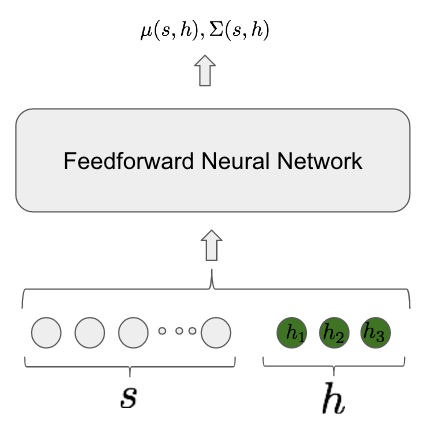
\includegraphics[width = 0.2\textwidth]{Figures/architecture-concatenate-snn.png}
	}
	\subfigure[Bilinear interaction]{
		\centering
		\label{fig:snn_architecture_bilinear}
		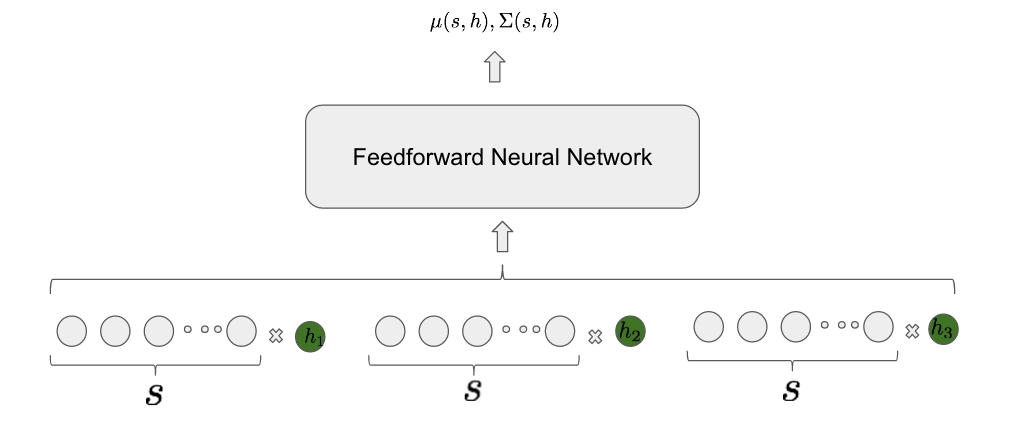
\includegraphics[width = 0.5\textwidth]{Figures/architecture_bilinear_snn.png}
	}
	\caption{Different architectures for the integration of the latent variables in a FNN}
	\label{fig:snn_architecture}
\end{figure}

The simplest joint embedding, as shown in Figure~\ref{fig:snn_architecture_concatenate}, is to concatenate the observations and the latent variables directly.\footnote{In scenarios where the observation is very high-dimensional such as images, we can form a low-dimensional embedding of the observation alone, say using a neural network, before jointly embedding it with the latent variable.} However, this limits the extent of interaction between the observation and latent variable. Richer forms of interactions, such as multiplicative interactions and bilinear pooling, have been shown to have greater representation power and improve the optimization landscape, achieving better results when complex interactions are needed \citep{fukui2016multimodal, wu2016multiplicative}. Inspired by this work, we study using a simple bilinear interaction, by forming the outer product between the observation and the latent variable. An illustration of this form of interaction is shown in Figure~\ref{fig:snn_architecture_bilinear}. As shown in the experiments, the choice of interaction greatly affects the quality of the span of skills that is learned. %alternative bilinear interaction bilinear integration between the observation inputs and the latent variables. 


Compared to training separate policies, training a single SNN allows for flexible weight-sharing schemes among different policies. Although the total number of parameters is larger compared to a single non-stochastic feed-forward policy due to the use of a joint embedding compared to an embedding of the observation alone, we will see below that SNNs results in a significant reduction in the sample complexity required to learn a rich set of skills.

In the pre-training environment, rather than re-sampling the latent variable at every time step, which will destroy the consistent behaviors by committing to the same skill, we use the same sampled latent code throughout the entire episode. After training, each of the latent code in the categorical distribution will correspond to a different skill, which can be then used for the downstream tasks.%fix the sampled latent variable throughout an episode. 

% ,As noted in many previous work \citep{fukui2016multimodal,  \cite{wu2016multiplicative}, For the joint embedding, We study two techniques for the joint embedding. As shown in the experiments, the choice of the embedding layer has a significant effect over the diversity of the learned skills.

%Special cases They have much larger capacity in representing multi-modal action distributions.


%distinct learned skills are rich enough

%needs to establish basic

%use them 


% \subsection{Using the pre-train MDP}
% Contrary to most MDPs reported in the literature, in our pre-train setup we want to have different optimal (even locally) solutions. Each of them will yield a possibly useful skill for the tasks to come. Hence a first method to obtain our span of skills is simply to solve several times this generic MDP and collect optimal policies. As will be seen in the Experiments section, this reward is enough to yield most of the interesting skills that a mobile robot should have. \textit{This will be our baseline?}

% Nevertheless, there are two main drawbacks to this straight-forward approach. First, the MDP has to be solved from scratch multiple times given that using part of the training of another policy will make them converge to the same local optima, hence not increasing the span of skills. This can become quite expensive in cases where this policy includes vision or is trained end-to-end [cite Chelsea?]. Second, training multiples policies independently complicates the task to motivate the diversity of the skills learned by each one of them. Therefore we propose to use the extra expressive power of Stochastic Neural Networks (SNNs) to address this two problems. As introduced in the preliminary work and in the appendix, SNNs are able to represent multi-modal distributions. And when used as policies to solve MDPs, this policy can also becomes multi-modal and each of these modes can later be used as a skill. Furthermore, as described in the two following subsection, architecture and information-theoretic enhancements can be applied to encourage the diversity of skills. Therefore, without increasing the difficulty of the pre-training procedure we get a more effective span of skills than training multiple policies separately.

% MENTION: For training, at the begining of the rollout, we sample a latent uniformly and fix it. Also mention the changes in the training algorithm. Should this be an extra sub-section? 

% \subsection{Impact of the SNN architecture}
% As introduced in the preliminary material, Stochastic Neural Networks can take many different forms, as long as they have some latent variables that are channeled through the non-linearities. For the purpose of learning different skills we have found most convenient to use discrete latent variables so that the modes are easily isolated and interpretable. Therefore we use latents being $h\sim \mathbb{P}_h$ where $\mathbb{P}_h$ is a categorical distribution yielding one-hot vectors. Note that other distributions could be chosen, including continuous, without affecting any of the other aspects of the our framework.

% Given the critical importance of learning a wide span of skills, we report two variants of the integration of the latent variables in a Feedforward Neural Network. The architecture choice has a high impact on the variety and interpretability of the representations learned. The simplest integration of the latent variables is to concatenate them with the actual observation at the input of the FNN. A wider impact on the architecture can be achieved by using bilinear integration of the observation source and the latent code source before inputing it to the FNN. See Fig. \ref{fig:snn_architecture} for a graphical representation of the two architectures. 

% Note that the bilinear integration with one-hot vectors as proposed in Fig.\ \ref{fig:snn_bilinear} can be interpreted as changing the whole first layer of the FNN based on the latent code sampled. 

% Even with the additional parameters needed to accomodate the enlarged input, SNNs are still much cheaper in parameters than training independent policies.\textit{ Re-trying only the first layer from the different policies trained sequentially will not grant a larger span of skills as most tries will fall in the same optima. <-- I have not checked that.. and even if I do, would I report that? Should this go in the experiments all together?}

% \textit{This modification already yields a high span of skills so we haven't tried more/Other integrations could be explored}.

% \subsection{Policy Optimization with Stochastic Neural Networks}
% \label{section:method:snnpolopt}

% Although SNNs have far richer representation power than 

\subsection{Information-Theoretic Regularization}
\label{section:method:inforeg}

Although SNNs have sufficient expressiveness in representing multi-modal policies, there is nothing in the optimization that prevent them from converging onto a single mode. Although we have not observed this worst case scenario in our experiments, we do find that sometimes different (discrete) latent variables correspond to the same or very similar skills. It is desirable to have direct control over the diversity of skills that will be learned. To achieve this, we introduce an information-theoretic regularizer, inspired by recent success of similar objectives in encouraging interpretable representation learning in GANs \citep{chen2016infogan}.

We design this objective specifically for mobile robots, although in principle it can be also generalized to other contexts.
%%TODO: briefly discuss this?
Concretely, we add an additional reward bonus, proportional to the mutual information between the latent variable and the state it is currently in. We only measure the mutual information with respect to a relevant subset in the state. For a mobile robot, we choose this to be the coordinates of its center of mass. We further partition the coordinate space into discrete grids, and map the continuous-valued coordinate into the closest grid. This way, calculation of empirical mutual information only requires maintaining counts of the latent variables in each grid.

Mathematically, let $X$ be a random variable denoting the grid in which the agent is currently situated, and let $Z$ be a random variable for the latent variable. Our additional reward bonus is $\alpha_H I(Z;X) = \alpha_H (H(Z) - H(Z|X))$, where $H$ denotes the entropy function. In our case, $H(Z)$ is constant since the distribution of the latent variable is fixed, and hence maximizing mutual information is equivalent to minimizing the conditional entropy. Therefore, another interpretation of this bonus is that given where the robot is, it should be easy to infer what skill the robot is currently performing. %latent variable 
%%PA: add something about how this is done? e.g. is a classifier being trained to do so, and does its performance affect reward? 

% involves simple reduces , which is a very weak form of We preserve visitation frequency of the mobile robot over a grid partition of the coordinate space, where the resolution of the grid is a hyperparameter. The intuition behind this bonus is that different values of the latent variable should induce different visitation patterns, which in turn corresponds to different skills. Formally, let $q$ be coordinates of a single grid, and let $h$ be a latent variable. %a variable representing a %will encourage different skills to be learned.

% discretized 

% To further encourage the diversity of skills learned while training a SNN we introduce an information-theoretic based intrinsic reward. If many latents produce a motion of the robot towards the same region, it will be hard to infer what was the latent sampled at the beginning of the trajectory. Hence we can give a reward to every state based on how easily the latent is inferred. Formally we use the trajectories from the batch (and their latent) to obtain an empirical estimate of the posterior distribution $p(h|s)$ over latents given a state. Then the reward obtained in any sampled state $s_t$ is modified by $-\alpha_H H(p(h|s_t))$, where $\alpha_H$ is an hyperparameter that modulates the weight of this bonus. In parctice, this computation can be done very efficiently by gridding the space and counting the number of times each latent visited each grid. \textit{introduce the grid meshing hyperparameter here?}. Then the posterior $p(h_i|s_t)$ is simply taken as the ration of frequencies between the number of times states belonging to trajectories with latent $h_i$ visited the cell $n_h$ and total visitations of the cell $n_T$. Then the reward becomes $-\log(\frac{n_h}{n_T})$. \textit{Review this, specify better that the state is associated to the cell, and then put super-scripts to the $n$s}

\subsection{Learning High-level Policies}
\label{section:method:highlevel}

Given a span of skills learned from the pre-training task, we now describe how to use them as basic building blocks for solving tasks where only sparse reward signals are provided. Assuming that the categorical latent variable has $K$ classes, and hence there are $K$ different skills, the high-level policy operates by selecting among these different skills. For a given task $M \in \mdpset$, and given a known factored representation of the state space $\sset^M$ as $\sset_\agent$ and $\sset_{\mathrm{rest}}^M$, the high-level policy receives the full state as input, and outputs a discrete action out of $K$ possible choices. The high-level policy operates at a slower time scale than the SNN policy, and we denote this time scale by $\tau$, a hyperparameter to be determined based on the downstream task. We choose to parametrize the high-level policy as a separate neural network for each MDP. We freeze the weights of the SNN during this phase of training, and we show in the experiments that this is already sufficient to achieve good performance in the downstream tasks. In principle, they can also be jointly optimized to adapt the skills to the task at hand. %while training We choose to represent the 

\subsection{Policy Optimization}
\label{section:method:polopt}

For both the pre-training phase and the training of the high-level policies, we use Trust Region Policy Optimization (TRPO) as the policy optimization algorithm \citep{Schulman15TRPO}. We choose TRPO due to its excellent empirical performance and because it does not require excessive hyperparameter tuning. For the pre-training phase, the training of policies is complicated by the fact that due to the presence of latent variables, the marginal distribution of $\pi(a|s)$ is now a mixture of Gaussians instead of a simple Gaussian, and it may even become intractable to compute if we use more expressive latent variables. This also complicates the computation of KL divergence, which is needed to control the step size of the policy update. In our implementation, we hold the latent variable as fixed in the optimization phase, and compute $\pi(a|s,z)$, where $z$ is the latent variable, without marginalizing over $z$. The rest of the TRPO procedure can then be straightforwardly applied. %treat the latent variable as part of the observation to the policy, stochastic 






% The MDPs that we want to tackle have a highly sparse reward structure and trying to learn a good policy from scratch in that environment can take very long or be not possible for standard methods. We propose to use the skills learned in the pre-training task in a hierarchical way to overcome this difficulty and learn faster. Instead of learning the low level skills again, we propose to learn only how to select skills sequentially. To do so we introduce a new "Pilot/Operator/high-level/manager" policy $\mathcal{M}_i$ for each new MDP $m_i$. This policy receives as input the full state $s_t\in \mathcal{S_i}$ and outputs a one-hot vector of dimension equal to the number of pre-trained skills. This vector is then used to select a skill to be active for the following $T_{agg}$ steps. During this time the actions takes are exclusively based on the robot observations $s^R_t\subset s_t$ and the active skill, and given that $\mathcal{A}_i = \mathcal{A}_{in}$ these actions can directly be applied to the current MDP $m_i$.


% For the multi-policy architecture, each entry of the one-hot is used to multiply the output of each of the pre-trained policies. Summing this weighted/masked outputs effectively yields the action corresponding to the selected skill. For the SNN architecture, the one-hot vector is directly inputed in place of the latent. See details in Fig.\ \ref{fig:snn_architecture}

% Our implementation parametrized the categorical distribution of the manager with a Neural Network with a soft-max at the output. The pre-trained networks remain fixed during learning in the new MDP $m_i$, therefore despite sampling a discrete variables we can still obtain the derivative of the policy with respect to all the trainable parameters with standard back-propagation and any policy gradient algorithm can be used to train the manager network. In fact, given now the discrete nature of the output of the trainable part, other methods like DQN or even value iteration could be used, opening a new realm of possibilities. We will still use TRPO just for simplicity/coherence/??. \textit{should this already be in experiments?}


\section{Experiments}

% We apply our framework to a collection of navigation tasks proposed b \cite{duan2016benchmarking}. Here, the agent controls a 3-link swimmer to navigate 

We have applied our framework to solving with a 3-link swimmer four mazes and a gathering task. Mazes 0 and 1 are depicted in Fig.\ \ref{fig:Maze0}-\ref{fig:Maze1}, where the robot is shown in its starting position and has to reach the other end of the U turn. Mazes 2 and 3 are different instantiations of the environment shown in Fig.\ \ref{fig:Maze2}, where the goal has been placed in the North-East or in the South-West corner respectively. A reward of 1 is only granted when the robot reaches the goal position. In the gathering task, the robot gets a reward of 1 for collecting green balls and a reward of -1 for the red ones, all of which are positioned randomly at the beginning of each episode. The sensor readings for the mazes and the latter task are fully described in the benchmark of continuous control problems \citep{duan2016benchmarking}, where it was shown that algorithms that employ naive exploration strategies could not solve them. Our hyperparameters for our Neural Networks and algorithms are detailed in the appendix.

\begin{figure}[h!]
	\centering
	\subfigure[Maze 0]{
		\centering
		\label{fig:Maze0}
		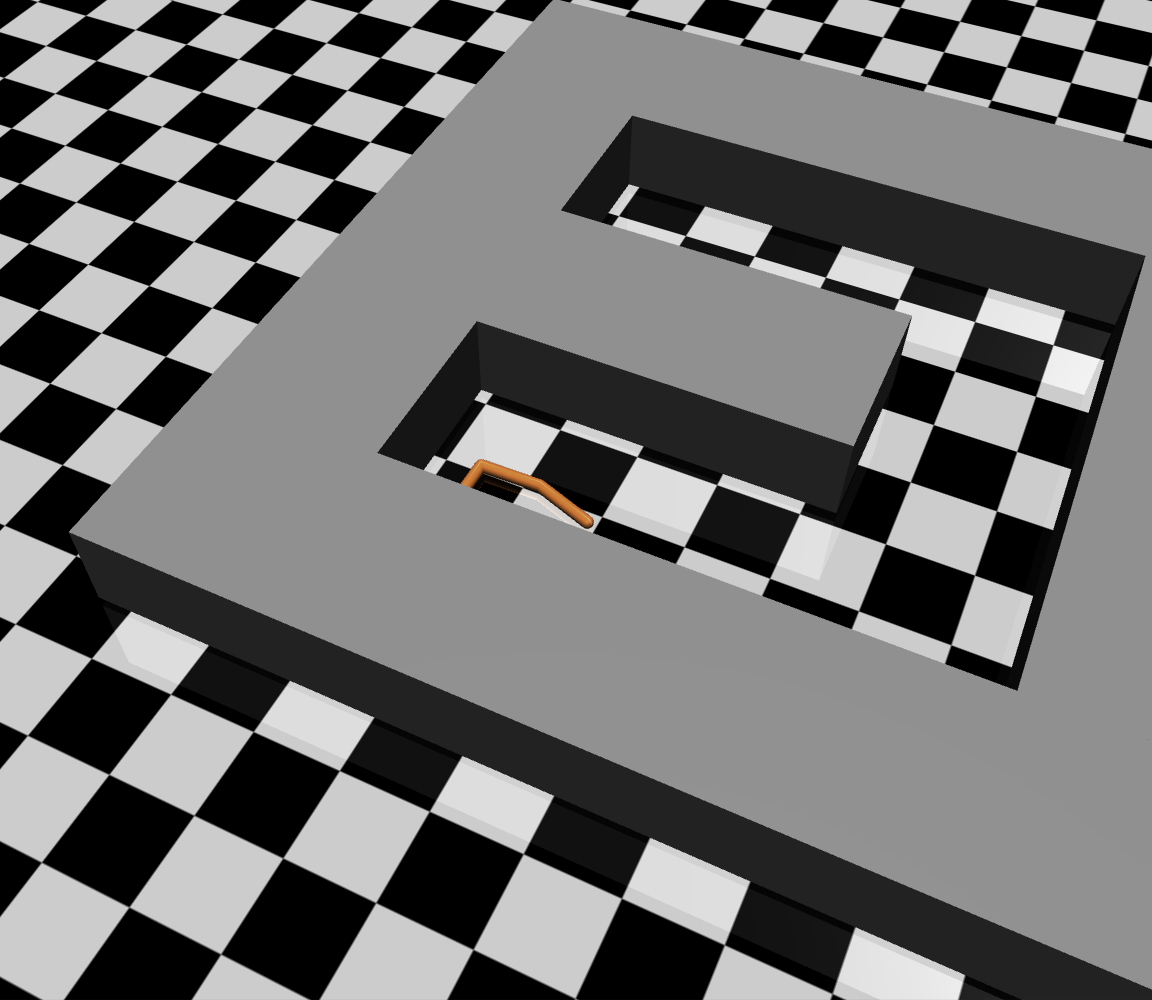
\includegraphics[width = 0.2\textwidth, height=0.2\textwidth]{Figures/Maze0.png}
	}
	\subfigure[Maze 1]{
		\centering
		\label{fig:Maze1}
		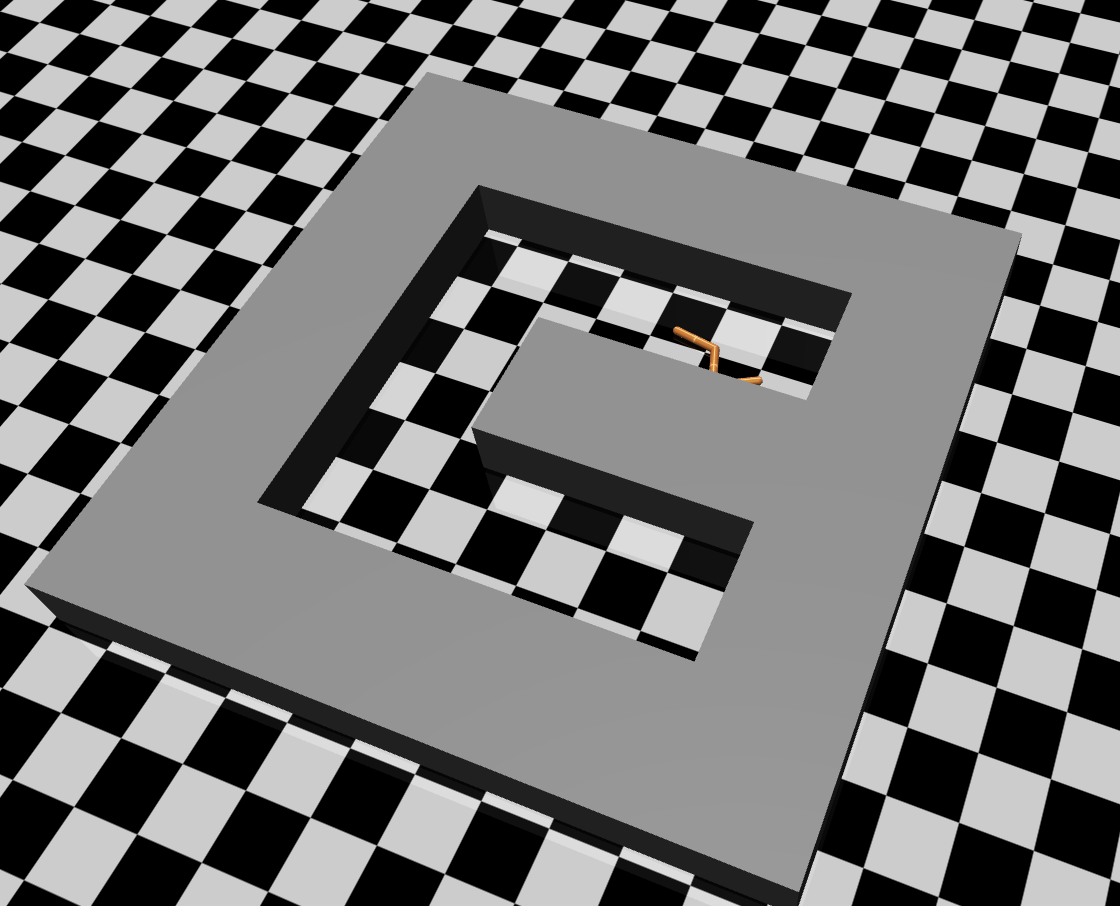
\includegraphics[width = 0.2\textwidth, height=0.2\textwidth]{Figures/Maze10.png}
	}
	\subfigure[Maze 2 or 3]{
		\centering
		\label{fig:Maze2}
		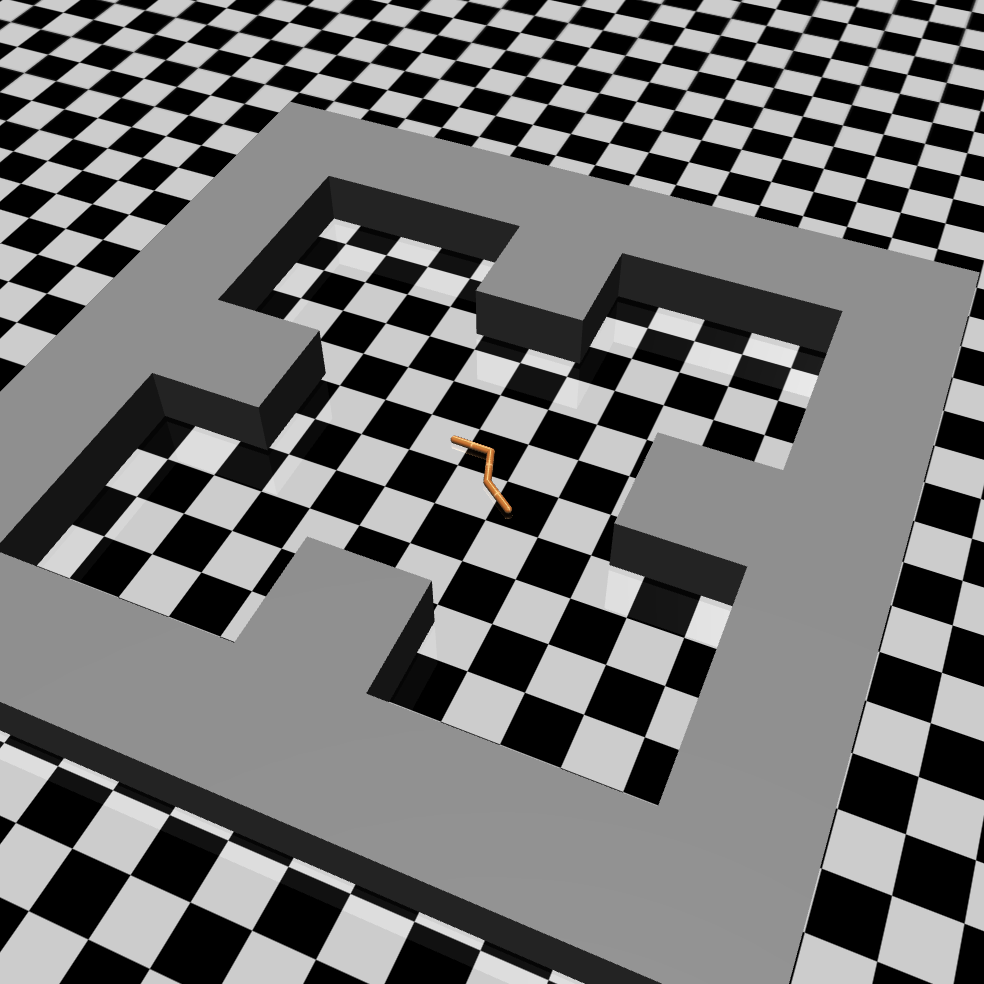
\includegraphics[width = 0.2\textwidth, height=0.2\textwidth]{Figures/Maze4.png}
	}
	\subfigure[Food Gather]{
		\centering
		\label{fig:FoodGather}
		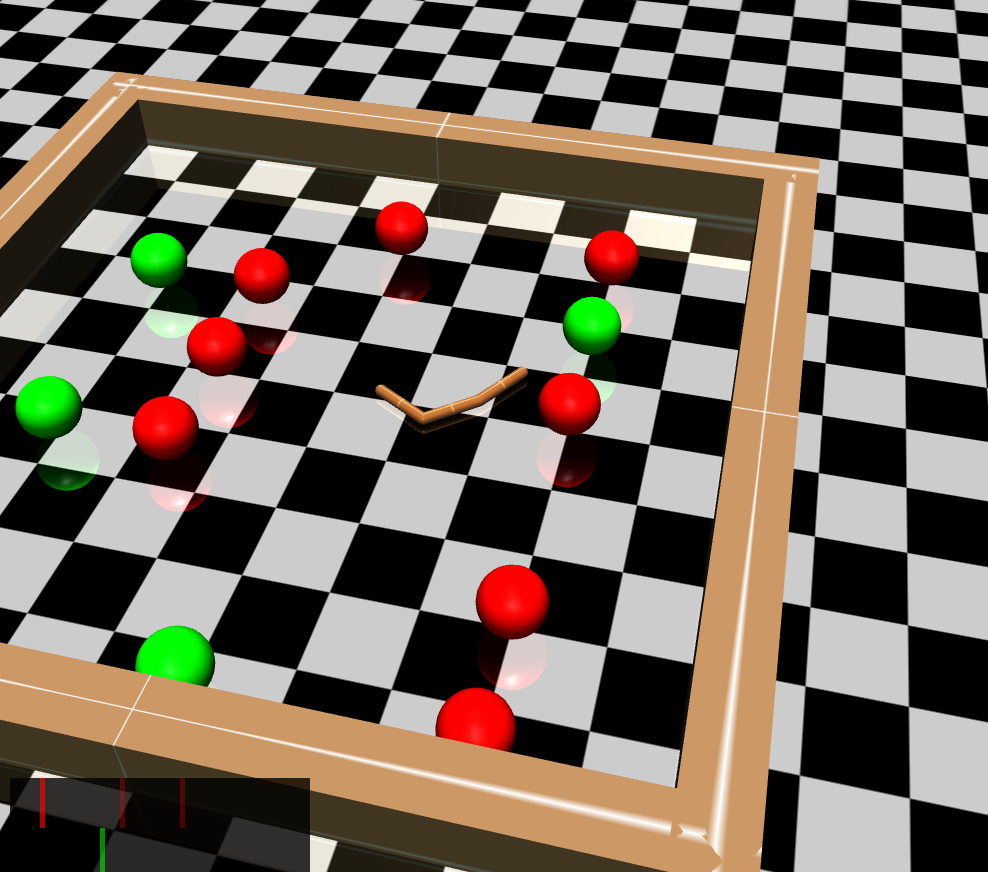
\includegraphics[width = 0.2\textwidth, height=0.2\textwidth]{Figures/FoodGatherSwimmer.png}
	}
	\caption{Illustration of the sparse reward tasks}
	\label{fig:snn_multimodal_MI}
\end{figure}


\section{Results}

First we evaluate the skill learning process, showing the relevance of the different pieces of our architecture and how they impact the exploration achieved when using them in a hierarchical fashion. Then we report the results on the sparse environments described above. We seek to answer the following questions:
\begin{itemize}
    \item Does pre-training with a intrinsic motivation reward yield a useful span of skills? Is it possible to consistently obtain a large span of skills without having to train the policies independently?
    \item Can the pre-training experience be leveraged to improve the exploration in downstream environments?
    \item Does the enhanced exploration help to solve sparse complex tasks such as mazes?
\end{itemize}

\subsection{Skill learning}

To evaluate the diversity of the learned skills we will use ``visitation plots'', showing the $(x,y)$ position of the robot's Center of Mass (CoM) during 100 rollouts of 500 steps each. In Fig.\ \ref{fig:visit-trpo-individuals} we show the visitation plot of 6 different policies, each trained from scratch in our pre-training environment. This yields 6 different ways of ``solving'' it. For better graphical interpretation and comparison with the next plots of the SNN policies, Fig.\ \ref{fig:visit_trpo6_likeSNN} shows a batch of 50 rollout for each of the 6 policies, each with a different color. Given the morphology of the swimmer, it has an natural preference for forward and backward motion so when no extra incentive is added, the visitation concentrates heavily on the direction it is initialized with.

The leftmost image of Fig.\ \ref{fig:visit_snn6_bilinear} shows the visitation plot of a SNN with bilinear integration and we see how it already has several ``skills''. Note how each latent generates a clearly interpretable behavior, despite not having any incentive to do so, other than the architecture itself. These skills may overlap more or less but we have observed that 80\% of the trained SNNs acquire at least forward and backward motion associated with different latents. On top of that, more turning skills than in Fig.\ \ref{fig:visit_trpo6_likeSNN} are observed, but without much consistency.

To improve upon this, we evaluate the impact of using the bilinear integration of the latent variables and the Mutual Information bonus. Fig.\ \ref{fig:visit_snn6_noBilinear} and \ref{fig:visit_snn6_bilinear} show, for concatenation and bilinear integration respectively, the visitation plots obtained with increasing values of the bonus coefficient $\alpha_H$. Using the Mutual Information bonus but not the bilinear integration also yields non-overlapping trajectories but it less consistentely yields a forward and backward motion as observed in Fig.\ \ref{fig:visit_snn6_noBilinear}. Without bilinear integration the latents cannot have a high level impact in the SNN and they are restricted to milder variations of a certain motion.
    
\begin{figure}[h]
	\centering
	\label{fig:visit-trpo-individuals}
	\subfigure[Independently trained policies in the pre-train MDP with the intrinsic reward of the CoM speed norm]{
		\centering
		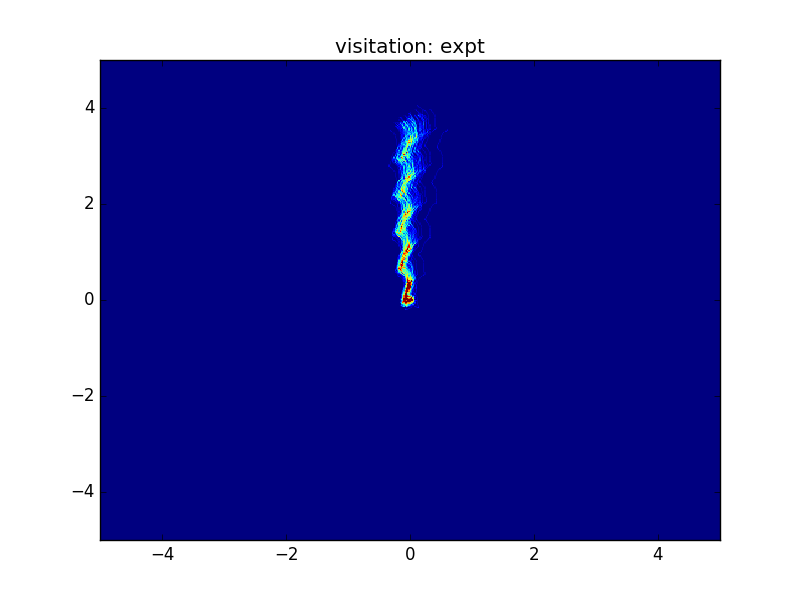
\includegraphics[trim={2cm 0 2cm 1.5cm}, clip, width=0.1\textwidth]{Figures/visit-trpo1.png}
	    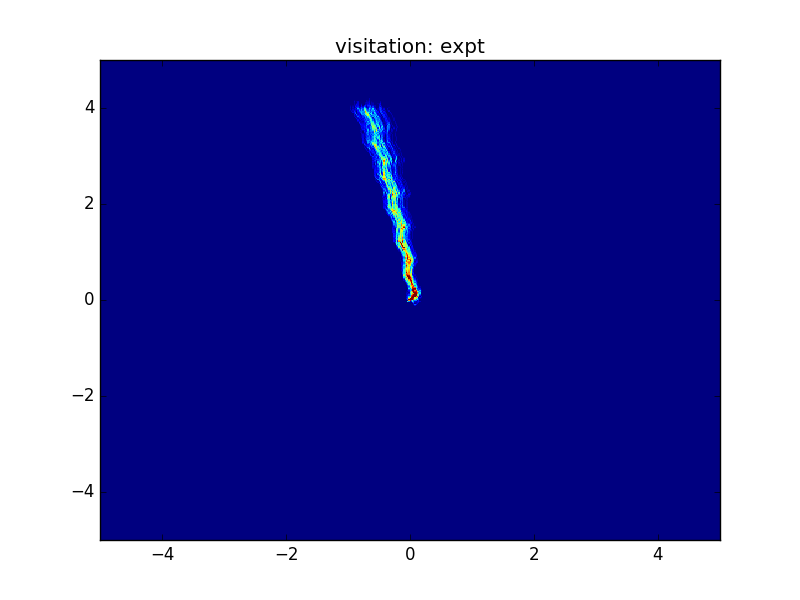
\includegraphics[trim={2cm 0 2cm 1.5cm}, clip, width=0.1\textwidth]{Figures/visit-trpo2.png}
		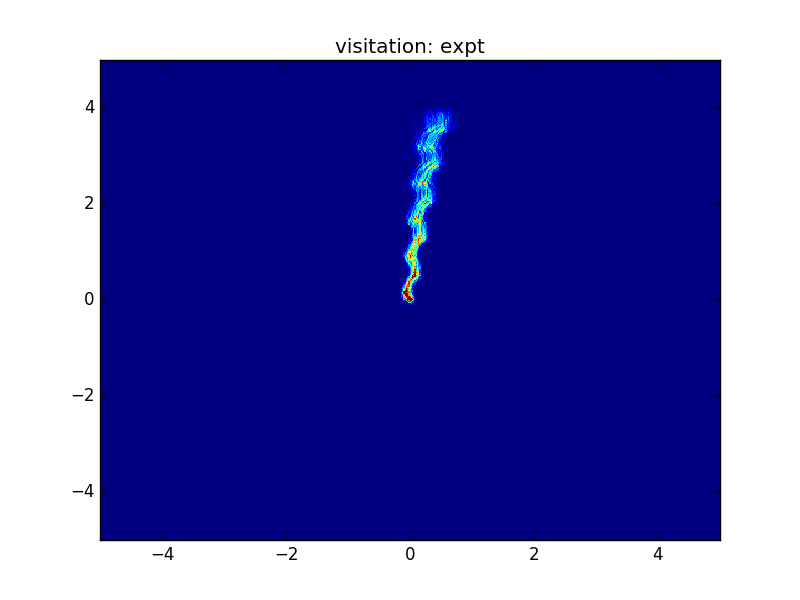
\includegraphics[trim={2cm 0 2cm 1.5cm}, clip, width=0.1\textwidth]{Figures/visit-trpo3.png}
	    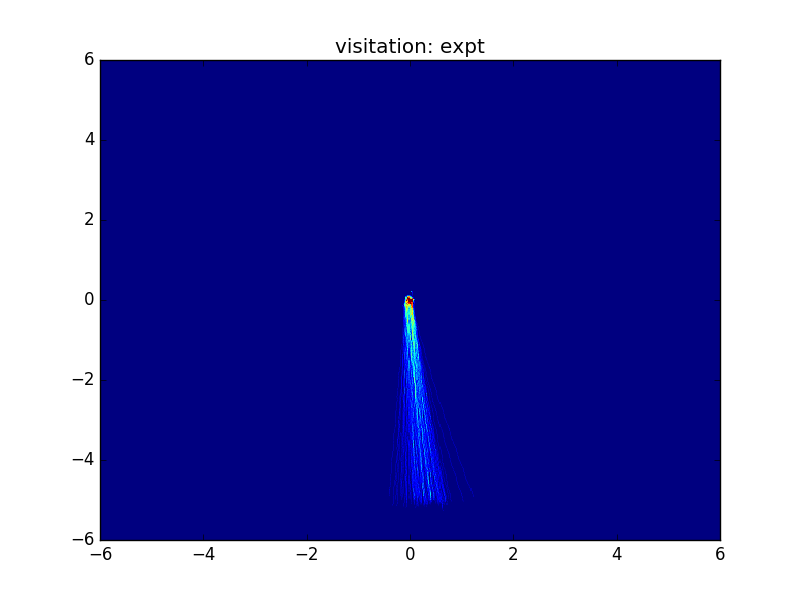
\includegraphics[trim={2cm 0 2cm 1.5cm}, clip, width=0.1\textwidth]{Figures/visit-trpo4.png}
		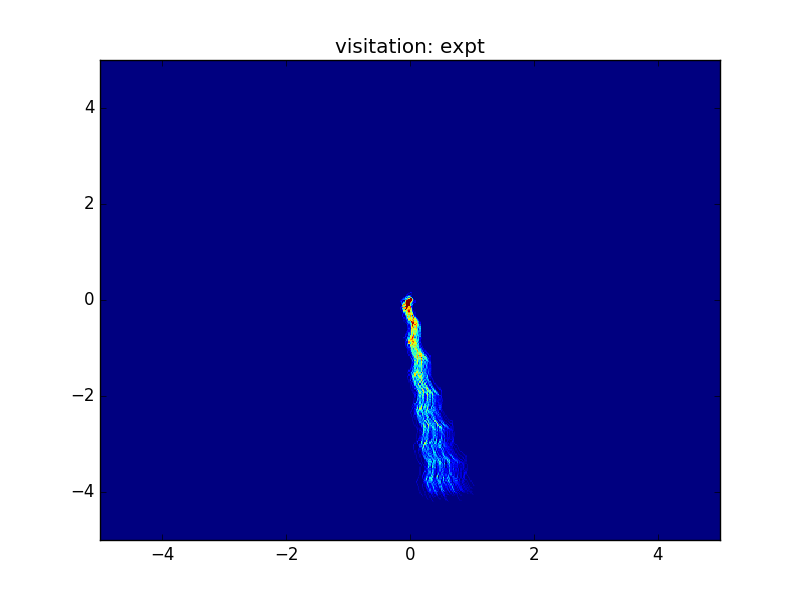
\includegraphics[trim={2cm 0 2cm 1.5cm}, clip, width=0.1\textwidth]{Figures/visit-trpo5.png}
	    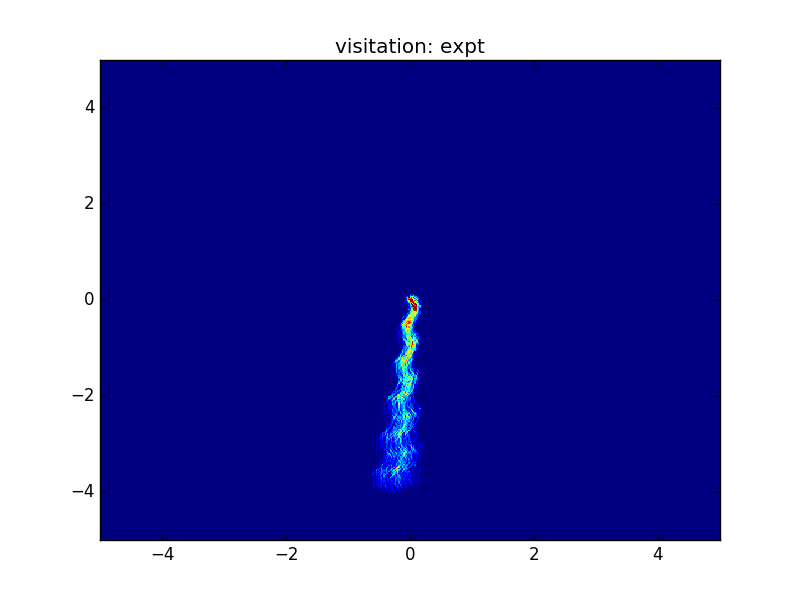
\includegraphics[trim={2cm 0 2cm 1.5cm}, clip, width=0.1\textwidth]{Figures/visit-trpo6.png}
	}
	\subfigure[Combined visitation of the independently trained policies from (a)]{
		\centering
		\label{fig:visit_trpo6_likeSNN}
	    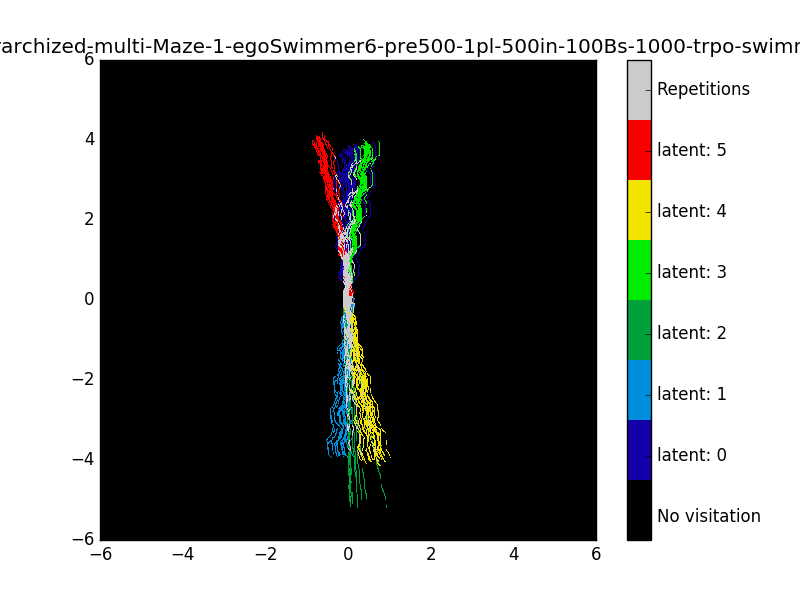
\includegraphics[trim={2cm 0 3.6cm 1.5cm}, clip, width=0.2\textwidth]{Figures/likeSNN-hierarchized-multi-Maze-1-egoSwimmer6-pre500-1pl-500in-100Bs-1000-trpo-swimmer-ego-500_visitation.png}
	}
	\subfigure[SNN \emph{without} bilinear integration and increasing $\alpha_H=0,0.001,0.01,0.1$]{
		\centering
		\label{fig:visit_snn6_noBilinear}
		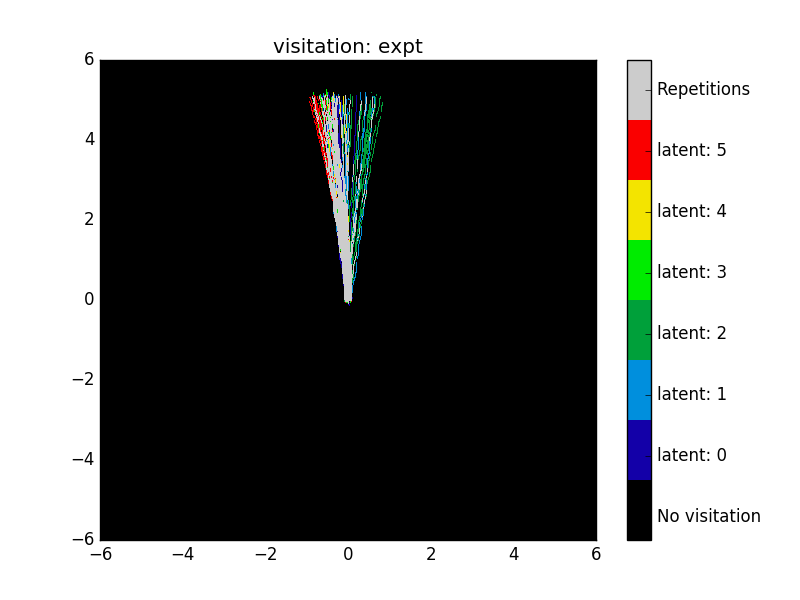
\includegraphics[trim={2cm 0 1cm 1.5cm}, clip, width = 0.2\textwidth]{Figures/visit-snn-NoBil-0MI.png}
		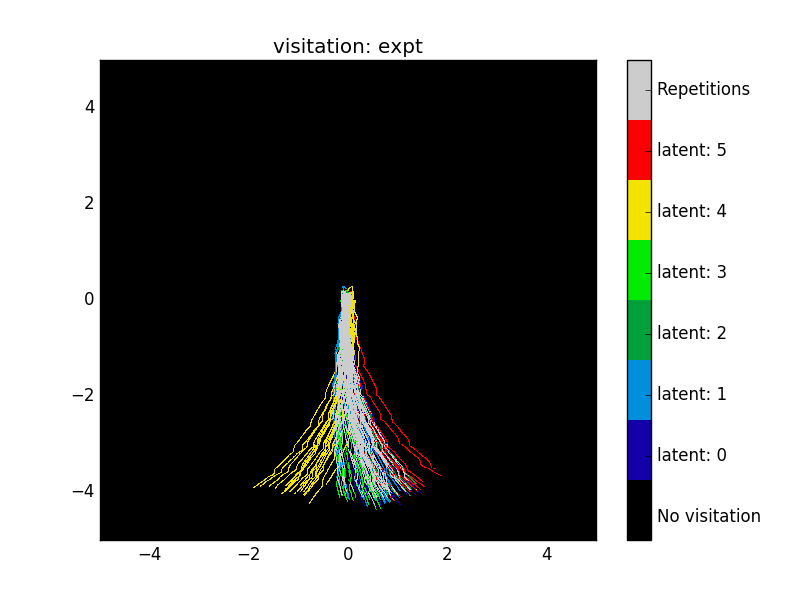
\includegraphics[trim={2cm 0 1cm 1.5cm}, clip, width = 0.2\textwidth]{Figures/visit-snn-NoBil-0001MI.png}
		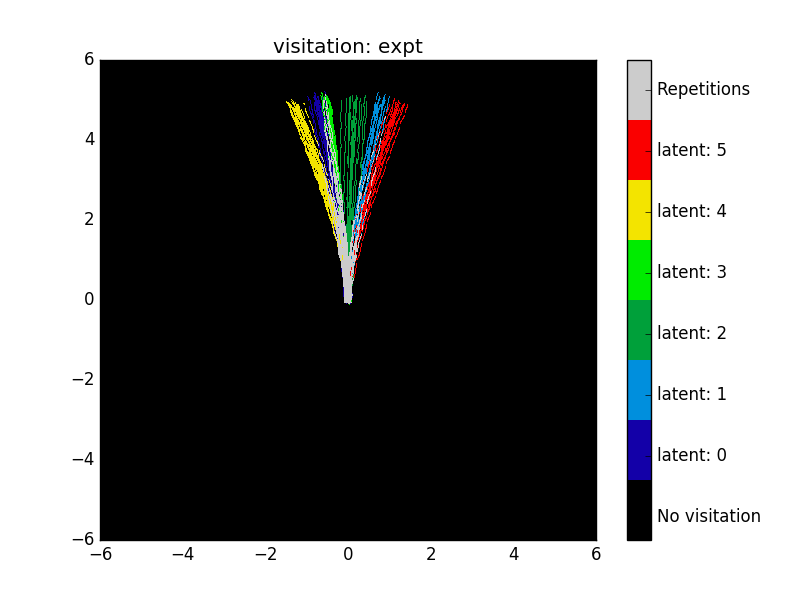
\includegraphics[trim={2cm 0 1cm 1.5cm}, clip, width = 0.2\textwidth]{Figures/visit-snn-NoBil-001MI.png}
		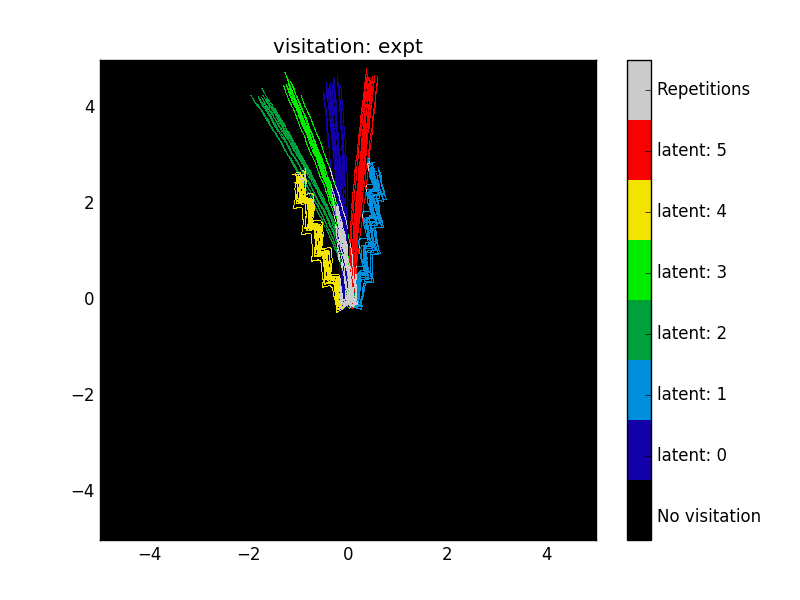
\includegraphics[trim={2cm 0 1cm 1.5cm}, clip, width = 0.2\textwidth]{Figures/visit-snn-NoBil-01MI.png}
	}
	\subfigure[SNN \emph{with} bilinear integration and increasing $\alpha_H=0,0.001,0.01,0.1$]{
		\centering
		\label{fig:visit_snn6_bilinear}
		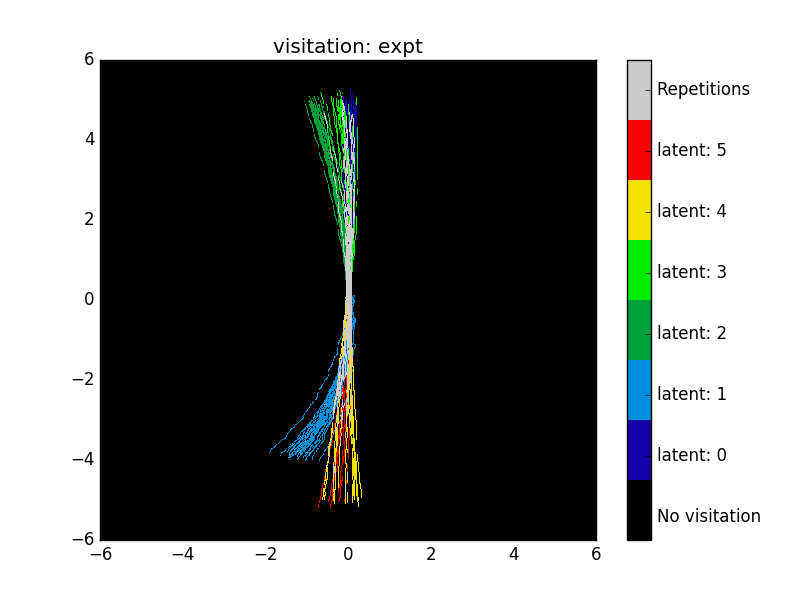
\includegraphics[trim={2cm 0 1cm 1.5cm}, clip, width = 0.2\textwidth]{Figures/visit-snn-Bil-0001MI.png}
		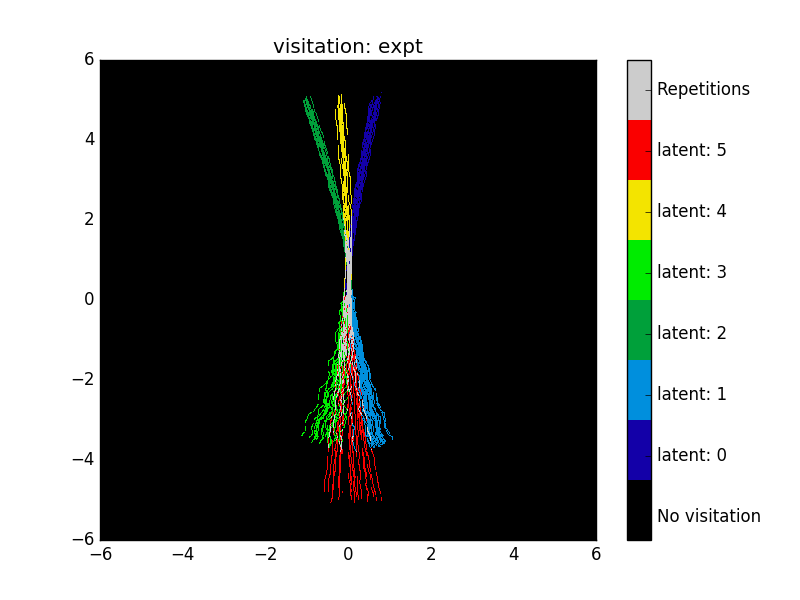
\includegraphics[trim={2cm 0 1cm 1.5cm}, clip, width = 0.2\textwidth]{Figures/visit-snn-Bil-001MI.png}
		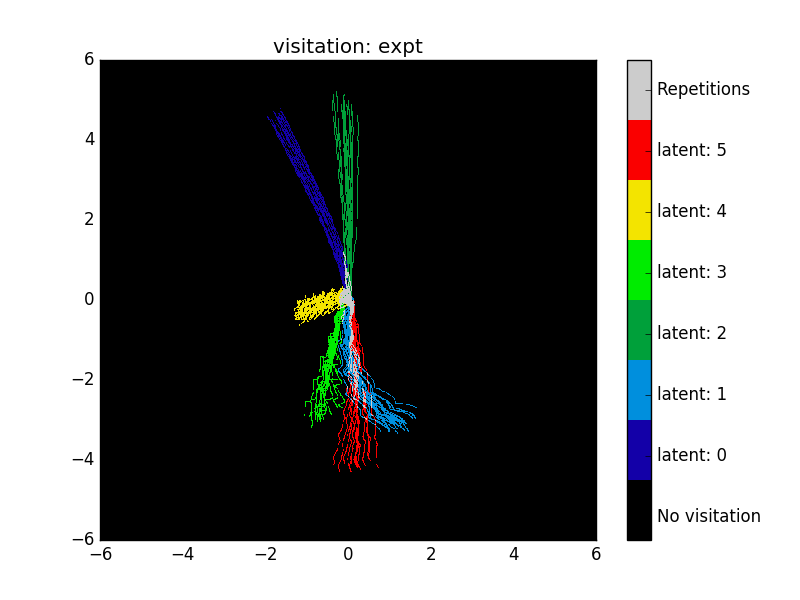
\includegraphics[trim={2cm 0 1cm 1.5cm}, clip, width = 0.2\textwidth]{Figures/visit-snn-Bil-01MI.png}
		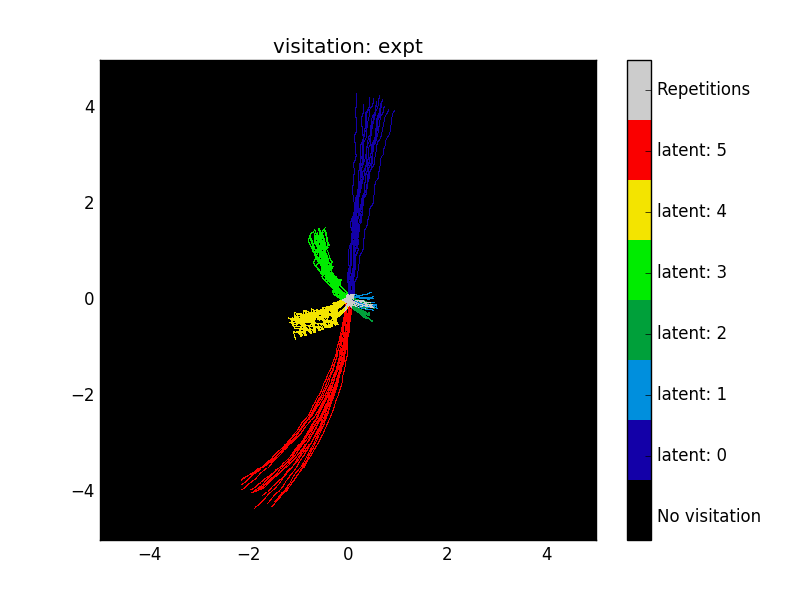
\includegraphics[trim={2cm 0 1cm 1.5cm}, clip, width = 0.2\textwidth]{Figures/visit-snn-Bil-1MI.png}
	}
	\caption{Span of skills learn by different methods and architectures}
	\label{fig:visit_methods}
\end{figure}


\subsection{Hierarchical use of skills}

The hierarchical architectures we propose have a very direct impact in the areas covered by random exploration. We will examine these with visitation plots of 100 rollouts of length 10.000 each. Fig.\ \ref{fig:visit-trpo-1M} corresponds to Gaussian noise at the output with $\mu=0$ and $\Sigma=I$, as usually used in the first iteration of policy gradient methods (like our pre-training task). The swimmer robot has actions clipped to $[-1,1]$, so this noise is relatively very large. In Fig.\ \ref{fig:visit-hier-multi-1M} we observe the drastic increase in exploration using the hierarchical approach with pre-trained policies. This plot shows a possible first iteration in the training of the manager network, hence being randomly initialize and picking policies almost uniformly, and committing to them for 500 steps before selecting the next one. The same setup for SNNs with bilinear integration and $\alpha_H= 0$ and 0.1 can be seen in Figs.\ \ref{fig:visit-hier-snnBil-1M} and \ref{fig:visit-hier-snnHB-1M} respectively. The exploration given by the multi-policy hierarchy concentrates quite heavily in upward and downword motion, as is expected form the individual policies composing it (Fig.\ \ref{fig:visit-trpo-individuals}). On the other hand the exploration obtained with SNNs yields a wider coverage of the space as the underlying policy usually has additional behaviors. Note how most of the latent changes of latent yield a corresponding change in direction.

\begin{figure}[h!]
	\centering
	\subfigure[Gaussian noise with covariance $\Sigma=I$]{
		\centering
		\label{fig:visit-trpo-1M}
		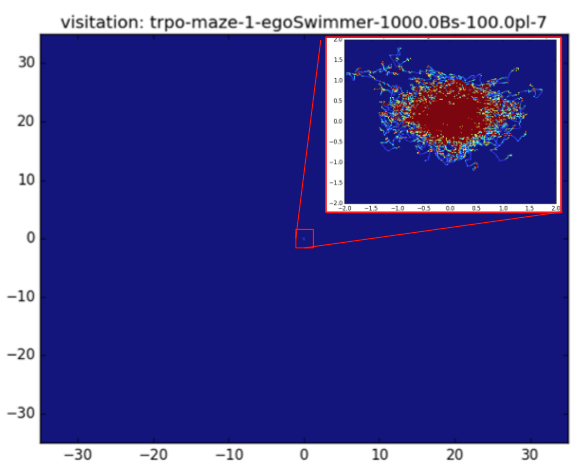
\includegraphics[trim={0cm 0 0cm 0cm}, clip, width = 0.22\textwidth]{Figures/visit-trpo-1M.png}
	}
	\subfigure[Hierarchichy with Multi-policy]{
		\centering
		\label{fig:visit-hier-multi-1M}
		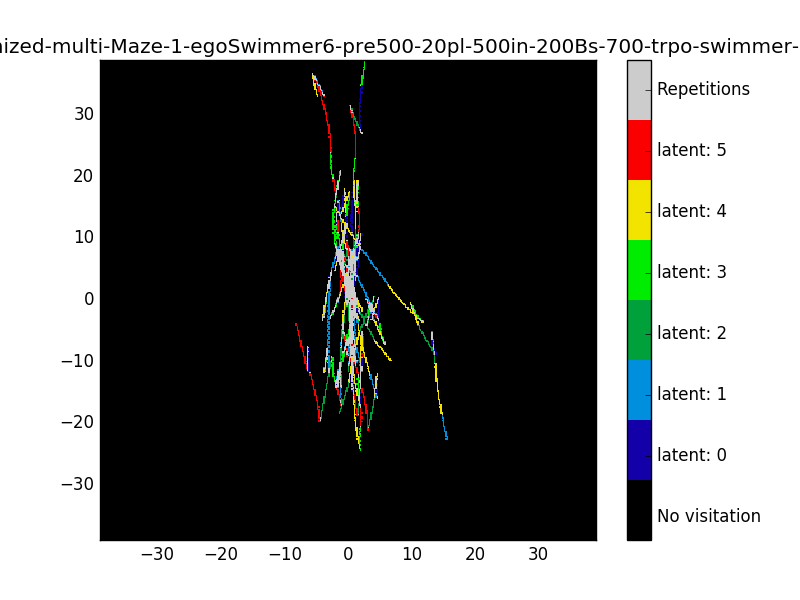
\includegraphics[trim={2cm 0 1cm 1.5cm}, clip, width = 0.22\textwidth]{Figures/visit-multi-2.png}
	}
	\subfigure[Hierarchy with Bilinear-SNN(,$\alpha_H=0$) ]{
		\centering
		\label{fig:visit-hier-snnBil-1M}
		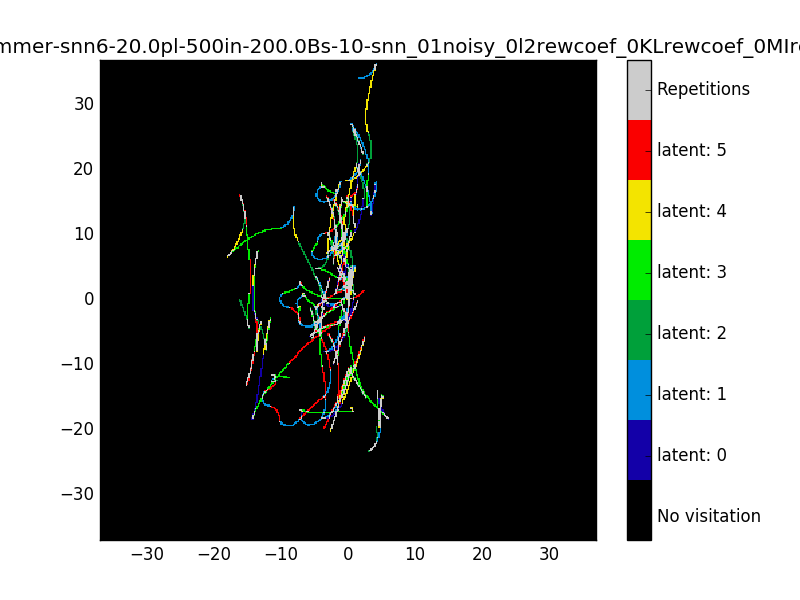
\includegraphics[trim={2cm 0 1cm 1.5cm}, clip, width = 0.22\textwidth]{Figures/visit-snn-1Mbisbis.png}
	}
	\subfigure[Hierarchy with Bilinear-SNN, $\alpha_H=0.01$]{
		\centering
		\label{fig:visit-hier-snnHB-1M}
		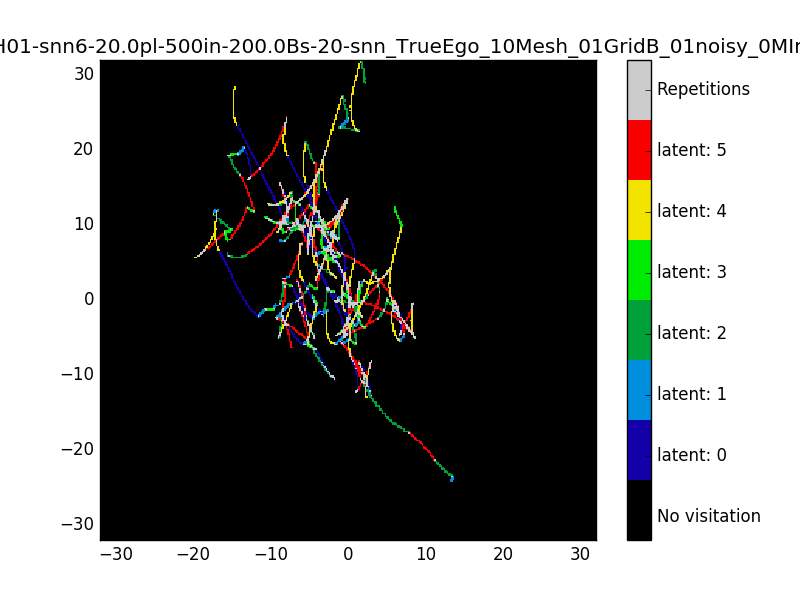
\includegraphics[trim={2cm 0 1cm 1.5cm}, clip, width = 0.22\textwidth]{Figures/visit-snnMI-1Mbis.png}
	}
	\caption{Visitation plots for different randomly initialized architectures (100 rollouts, 10k path length). All axis are in scale [-30,30] and we added a zoom for the Gaussian noise to scale [-2,2]}
	\label{fig:hierarchized-exploration}
\end{figure}

\subsection{Mazes and Gathering tasks}
Due to the sparsity of these tasks, none can be solved by standard reinforcement algorithms \citep{duan2016benchmarking}. In Fig.\ \ref{fig:learning-curves} we evaluate the different hierarchical architectures proposed. All the iterations are performed with rollouts of maximum path length of 10,000 samples and a total batch size of one million. We also compare them against a stronger baseline: adding to the downstream task the same intrinsic reward that was granted to the robot in the pre-training task. This baseline performs quite poorly in all the mazes, Fig.\ \ref{fig:learn-maze0}-\ref{fig:learn-maze4}. The hierarchical architectures are able to learn much faster in every new MDP. The benefit of using as hierarchy SNNs with bilinear integration is also clear over most mazes, although the Mutual Information bonus does not always boosts performance. We think that the extra skills will shine more in other tasks requiring more precise navigation. And indeed this is the case in the Gathering task as seen in Fig.\ \ref{fig:learn-gather}, where not only the average return increases but also the variance of the learning curve shrinks, denoting a more consistent training across different SNNs. The baseline of having an intrinsic reward in the task happens to be stronger than expected. Indeed, the task offers a not-so sparse reward, which can then be easily reached by an intrinsically motivated agent. In this case, the hierarchy may not be that useful and could even become a burden as it only allows the agent to change skill every 50 steps.

\begin{figure}[h!]
	\centering
	\subfigure[Maze 0]{
		\centering
		\label{fig:learn-maze0}
		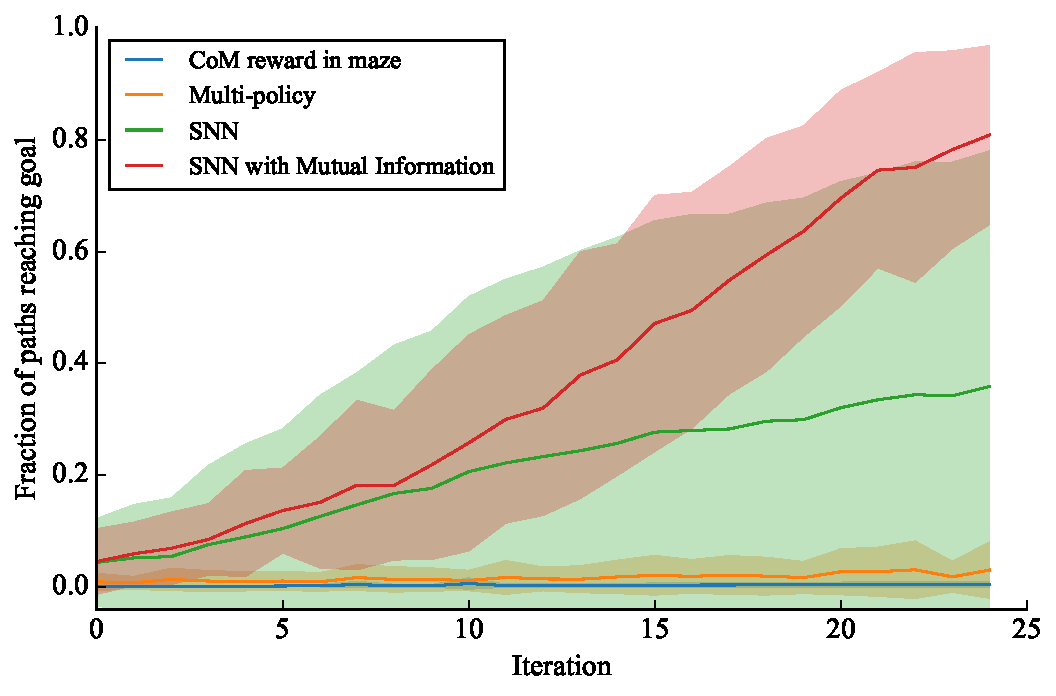
\includegraphics[width = 0.4\textwidth]{Figures/learning-Maze0.pdf}
	}
	\subfigure[Maze 1]{
		\centering
		\label{fig:learn-maze1}
		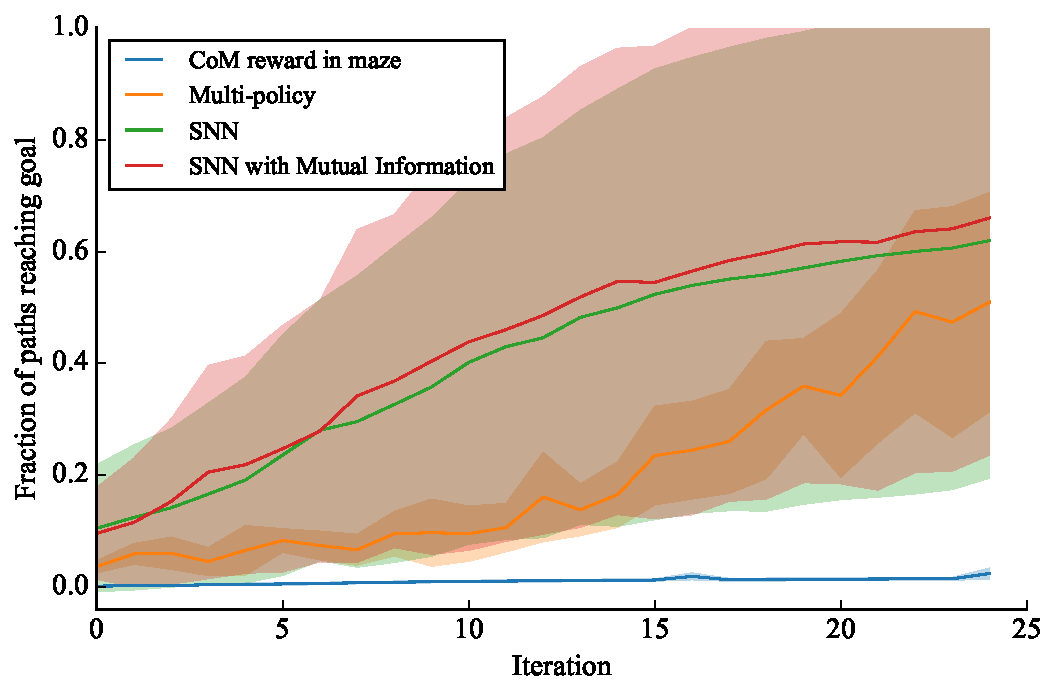
\includegraphics[width = 0.4\textwidth]{Figures/learning-Maze10.pdf}
	}
	\subfigure[Aggregated results for Mazes 2 and 3]{
		\centering
		\label{fig:learn-maze4}
		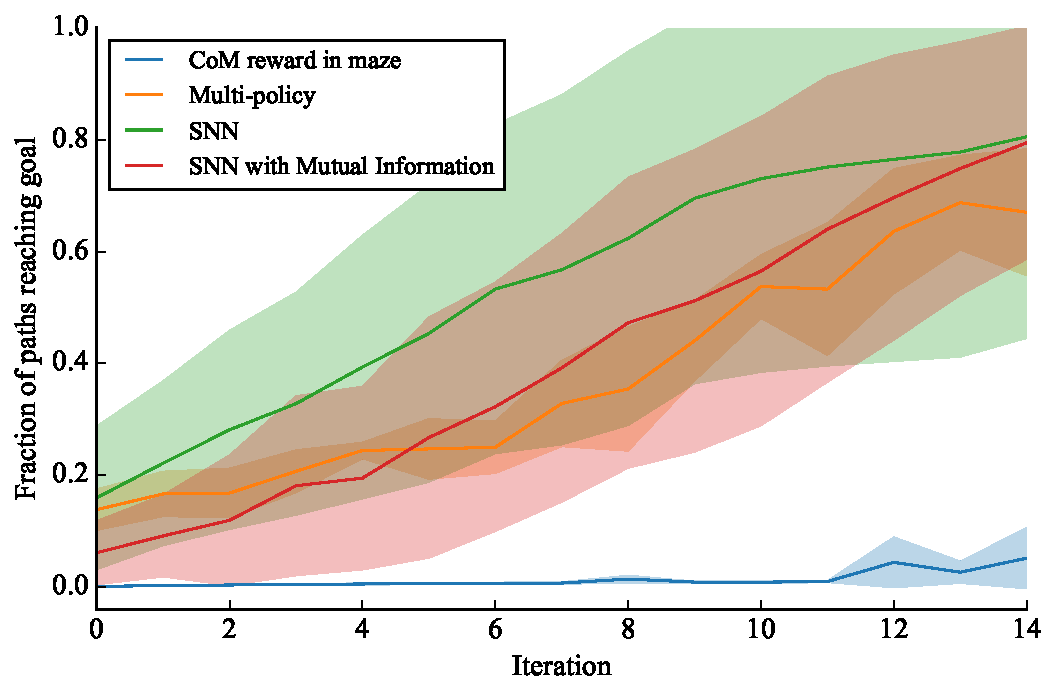
\includegraphics[width = 0.4\textwidth]{Figures/learning-Maze4.pdf}
	}
	\subfigure[Gathering task]{
		\centering
		\label{fig:learn-gather}
		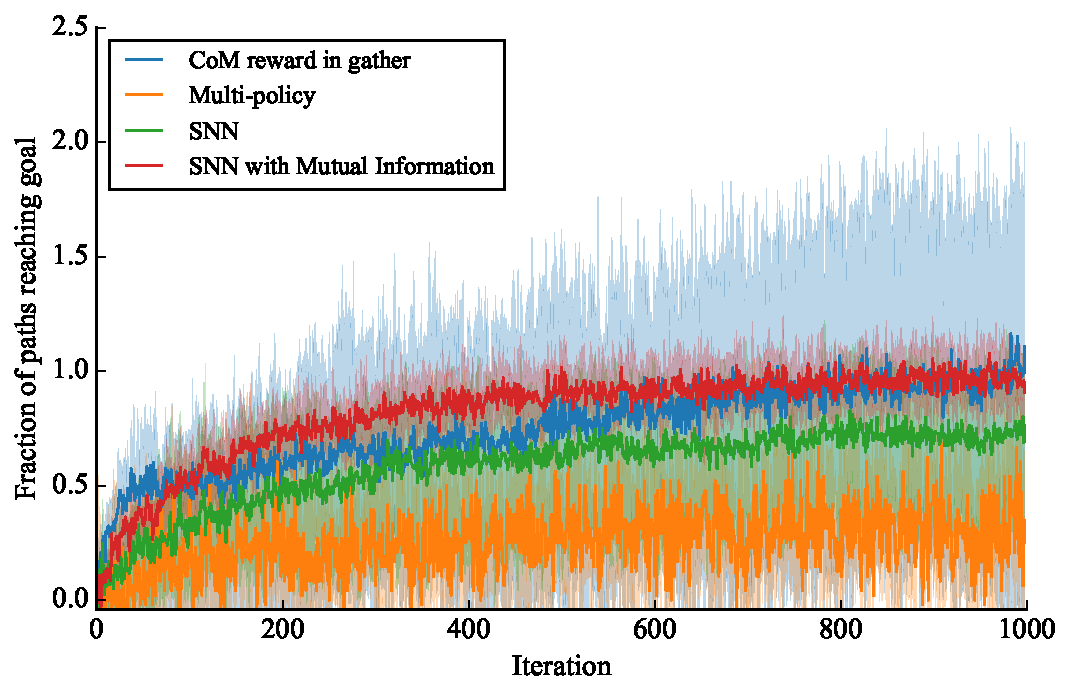
\includegraphics[width = 0.4\textwidth]{Figures/learning-Gather.pdf}
	}
	\caption{Fast learning of the hierarchical architectures in the new MDP tasks}
	\label{fig:learning-curves}
\end{figure}

\section{Discussion and future work}
We propose a setup that leverages, in an unsupervised way, the access to a limited agent-centric part of downstream MDPs to efficiently solve a collection of complex sparse reward tasks. Our framework successfully combines two parts, firstly an unsupervised procedure to learn a large span of skills using intrinsic motivation and secondly a hierarchical structure that encapsulates the latter span of skills and allows to re-use them in future tasks. The span of skills learning can be greatly improved by using stochastic neural networks as policies and their additional expressiveness and multimodality. Furthermore, we have studied how to improve the consistency of the learned diversity of behaviors by incorporating both architecture and training modifications that allow the latent variables to have a wider impact on the final policy learned. The bilinear integration and the Mutual Information are key to yield a wide, interpretable span of skills. As for the hierarchical structure, we demonstrate how drastically it can boost the exploration of an agent in a new environment and we demonstrate its relevance for solving complex tasks as mazes or gathering. The major limitations of our current approach is the fixed number of time-steps that the hierarchical manager commits to every behavior. Moreover, we only use Feedforward architectures and hence the decision of what skill to use next only depends on the observation at that moment, hence not using any sensory information that could have been gathered during that time. This issues could be alleviated by introducing a recurrent architecture at the manager level or b allowing the manager to terminate the commitment to the current skill, similar to the option framework.

\subsubsection*{Acknowledgments}
This work was supported in part by DARPA, the Berkeley Vision and Learning Center (BVLC), the Berkeley Artificial Intelligence Research (BAIR) laboratory, and Berkeley Deep Drive (BDD). This research was funded in part by ONR through a PECASE award. Carlos Florensa was also supported by the Ph.D. Fellowship of La Caixa - Spain. Yan Duan was also supported by a Berkeley AI Research lab Fellowship and a Huawei Fellowship.

\bibliography{ref}
\bibliographystyle{iclr2017_conference}

\appendix
\section{Hyperparameters}
The design parameters of our pre-train task and the next task are reported in Tab.\ \ref{tab:params}

\begin{table}[h!]
\centering
\begin{tabular}[t]{c|cc}
Parameter & multi-policy & SNN \\
\hline
number of skills $K$ & \multicolumn{2}{c}{6}\\
NN hidden units & \multicolumn{2}{c}{[32,32]}\\
Training algorithm & \multicolumn{2}{c}{TRPO}\\
Learning rate & \multicolumn{2}{c}{0.01}\\
Mesh size (for MI bonus)& \multicolumn{2}{c}{10}\\
\end{tabular}
\caption{Parameters of the model and algorithms}
\label{tab:params}
\end{table}

\end{document}
